% XeLaTeX can use any Mac OS X font. See the setromanfont command below.
% Input to XeLaTeX is full Unicode, so Unicode characters can be typed directly into the source.

% The next lines tell TeXShop to typeset with xelatex, and to open and save the source with Unicode encoding.

%!TEX TS-program = xelatex
%!TEX encoding = UTF-8 Unicode

\documentclass[12pt,oneside,a4paper]{report}
\usepackage[bookmarks=true, bookmarksopen=true, colorlinks=false, linkcolor=black, driverfallback=dvipdfm, pdfstartview=FitH, hidelinks]{hyperref}	%在PDF中增加Bookmaker

\usepackage{color}
\definecolor{bisque}{rgb}{.996,.891,.755}

\usepackage[top=2.5cm,bottom=2.75cm,left=2.5cm,right=2.5cm]{geometry}   %設定頁面留白

\usepackage[boldfont,slantfont,CJKnumber,CJKspace]{xeCJK}	%xeCJK套件
\usepackage{CJKnumb}
\setmainfont{Times New Roman}								%設定英文預設字體
\setCJKmainfont{標楷體}                                      %設定中文預設字體
\setCJKsansfont{標楷體}
% \setCJKmainfont{cwTeX Q Kai Medium}                       %若標楷體無法使用之中文預設字體
% \setCJKsansfont{cwTeX Q Kai Medium}citation

\usepackage{eso-pic}										%插入浮水印
\usepackage{graphicx}										%插入圖片
\usepackage[bf,indentfirst,pagestyles]{titlesec}			%定義章節名稱與文字型態
\usepackage{titletoc}										%定義章節名稱
\usepackage{cite}											%bibliography package
\usepackage{tabularx}
\usepackage{longtable}										%處理長表格
\usepackage{enumitem}
\usepackage{array}
\usepackage{float}
\usepackage{fancyvrb}
\usepackage{fancyhdr}
\usepackage[above]{placeins}
\usepackage{pstricks,pst-node,pst-tree}
\usepackage{wrapfig}
\usepackage{graphicx}
\graphicspath{ {./img/} }
\usepackage{caption}
\usepackage{subcaption}
\usepackage{multirow}
\usepackage{url}
\usepackage{listings}
\usepackage{color}
\usepackage{pdfpages}

\definecolor{light-gray}{gray}{0.95}

\lstset{basicstyle=\linespread{1.0}\ttfamily\footnotesize,
    backgroundcolor=\color{light-gray}, xleftmargin=0.7cm,
    frame=tlbr, framesep=0.2cm, framerule=0pt,
}
\setbox0=\hbox{\ttfamily}

%定義環境變數與巨集指令
%-------------------基本設定------------------------------------%
% 沿用 latex 的一些標點的轉換,如 en-dash 以兩個減號表示
\defaultfontfeatures{Mapping=tex-text}
\XeTeXlinebreaklocale "zh"
\XeTeXlinebreakskip = 0pt plus 1pt
%-------------------------------------------------------------%

%-------------------重新定義章節名稱格式--------------------------%
\titleformat{\chapter}[hang]{\centering\huge\bfseries}{第\CJKnumber{\thechapter}章}{1em}{}
%\renewcommand\chaptername{Chapter\hspace{.5em}\thechapter}
\renewcommand\contentsname{目錄}
\renewcommand\listfigurename{圖目錄}
\renewcommand\listtablename{表目錄}
\renewcommand\lstlistlistingname{程式碼目錄}
\newcommand{\loflabel}{圖} % 定義圖目錄顯示方式
\newcommand{\lotlabel}{表} % 定義表目錄顯示方式
\newcommand{\loclabel}{程式碼}

\titlecontents{chapter}[0pt]{}
    {第\CJKnumber{\thecontentslabel}章\quad}{}
    {\hspace{.5em}\titlerule*[10pt]{$\cdot$}\contentspage}
\titlecontents{section}[2em]{}
    {\thecontentslabel\quad}{}
    {\hspace{.5em}\titlerule*[10pt]{$\cdot$}\contentspage}
\titlecontents{subsection}[4em]{}
    {\thecontentslabel\quad}{}
    {\hspace{.5em}\titlerule*[10pt]{$\cdot$}\contentspage}

\renewcommand{\bibname}{參考文獻}            %修改參考文獻的標題名
\titlespacing{\chapter}{0pt}{*0}{*4}        %設定標題與四周的距離
\titlelabel{\thetitle\quad}				    %設定章節標題的樣式
\renewcommand{\figurename}{圖}
\renewcommand{\tablename}{表}
\renewcommand{\lstlistingname}{程式碼}
%-----------------------------------------------------------------%

%-------------------設定行距--------------------------------------%
\renewcommand{\baselinestretch}{2.1} % 大約等於word1.5倍行高

%設定enumerate等的item間距
\usepackage{enumitem}
\setenumerate{itemsep=-5pt}
\setitemize{itemsep=-5pt}
\setdescription{itemsep=-5pt}
%-----------------------------------------------------------------%

%-------------------定義浮水印------------------------------------%
\newcommand\WatermarkPicture{
   \put(0,0){
   \parbox[b][\paperheight]{\paperwidth}{
     \vfill
     \centering
     
\includegraphics[width=12.75cm,keepaspectratio]{watermark_ntut.png}%
     \vfill
     }
   }
}
%-----------------------------------------------------------------%

%------------------圖片巨集---------------------------------------%

%巨集格式
%mygraphic{圖片KeyWord}{圖片註解}{圖片路徑}
\def\myGraphic#1#2#3
{
	\begin{figure}[!htbp]
		\begin{center}
			\includegraphics[width=\textwidth]{#3}
			\caption{#2}\label{#1}
		\end{center}

	\end{figure}
}
%-----------------------------------------------------------------%

%------------------小小圖片巨集---------------------------------------%

%巨集格式
%mygraphic{圖片KeyWord}{圖片註解}{圖片路徑}
\def\myGraphicSS#1#2#3
{
	\begin{figure}[!htbp]
		\begin{center}
			\includegraphics[width=2cm]{#3}
			\caption{#2}\label{#1}
		\end{center}

	\end{figure}
}
%-----------------------------------------------------------------%

%------------------小圖片巨集---------------------------------------%

%巨集格式
%mygraphic{圖片KeyWord}{圖片註解}{圖片路徑}
\def\myGraphicS#1#2#3
{
	\begin{figure}[!htbp]
		\begin{center}
			\includegraphics[width=6cm]{#3}
			\caption{#2}\label{#1}
		\end{center}

	\end{figure}
}
%-----------------------------------------------------------------%

%------------------中圖片巨集---------------------------------------%

%巨集格式
%mygraphic{圖片KeyWord}{圖片註解}{圖片路徑}
\def\myGraphicM#1#2#3
{
	\begin{figure}[!htbp]
		\begin{center}
			\includegraphics[width=8cm]{#3}
			\caption{#2}\label{#1}
		\end{center}

	\end{figure}
}
%-----------------------------------------------------------------%

%------------------大圖片巨集---------------------------------------%

%巨集格式
%mygraphic{圖片KeyWord}{圖片註解}{圖片路徑}
\def\myGraphicB#1#2#3
{
	\begin{figure}[!htbp]
		\begin{center}
			\includegraphics[width=12cm]{#3}
			\caption{#2}\label{#1}
		\end{center}

	\end{figure}
}
%-----------------------------------------------------------------%

%------------------大大圖片巨集---------------------------------------%

%巨集格式
%mygraphic{圖片KeyWord}{圖片註解}{圖片路徑}
\def\myGraphicBB#1#2#3
{
	\begin{figure}[!htbp]
		\begin{center}
			\includegraphics[width=16cm]{#3}
			\caption{#2}\label{#1}
		\end{center}

	\end{figure}
}
%-----------------------------------------------------------------%

%------------------表格巨集---------------------------------------%
\renewcommand{\arraystretch}{1}

%巨集格式
%myTable{Table KeyWord}{Table註解}
\def\myTable#1#2
{
	\begin{table}[!htbp]
	\setlength{\abovecaptionskip}{0pt}
	\setlength{\belowcaptionskip}{10pt}
	\begin{center}
	\caption{#2}\label{#1}
}


\def\endmyTable
{
	\end{center}
	\end{table}
}

%-----------------------------------------------------------------%

%------------------修改圖與表的註解編號格式-----------------------%

\makeatletter
\long\def\@makecaption#1#2{%
  \vskip\abovecaptionskip
  \sbox\@tempboxa{{#1}\quad #2}%
  \ifdim \wd\@tempboxa >\hsize
    {#1}\quad #2\par
  \else
    \global \@minipagefalse
    \hb@xt@\hsize{\hfil\box\@tempboxa\hfil}%
  \fi
  \vskip\belowcaptionskip}
\makeatother

%-----------------------------------------------------------------%
%------------------修改Description縮排格式--------------------------%
%\makeatletter
%\renewenvironment{description}
%  {\list{}{\leftmargin\z@ \labelwidth\z@ \itemindent-\leftmargin
%   \let\makelabel\descriptionlabel}}
%  {\endlist}
%\makeatother
%-----------------------------------------------------------------%
%------------------Use Case巨集---------------------------------------%
%巨集格式
%useCase{UseCase名稱}{UseCase圖片路徑}
\def\useCase#1#2#3
{
	\subsection{#1}
	\begin{figure}[!htb]
		\begin{center}
			\includegraphics[width=\textwidth]{#2}
		\end{center}
	\end{figure}
}
% \graphicspath{{./picture/eps/}{./picture/png/}}
% \graphicspath{{.}}					%告訴Latex去這兩個目錄下找圖檔
%-----------------------------------------------------------------%
%-------------------為了方便所設定的巨集--------------------------%

%-----------------------------------------------------------------%


\begin{document}

\includepdf[pages={1}]{bookname.pdf}
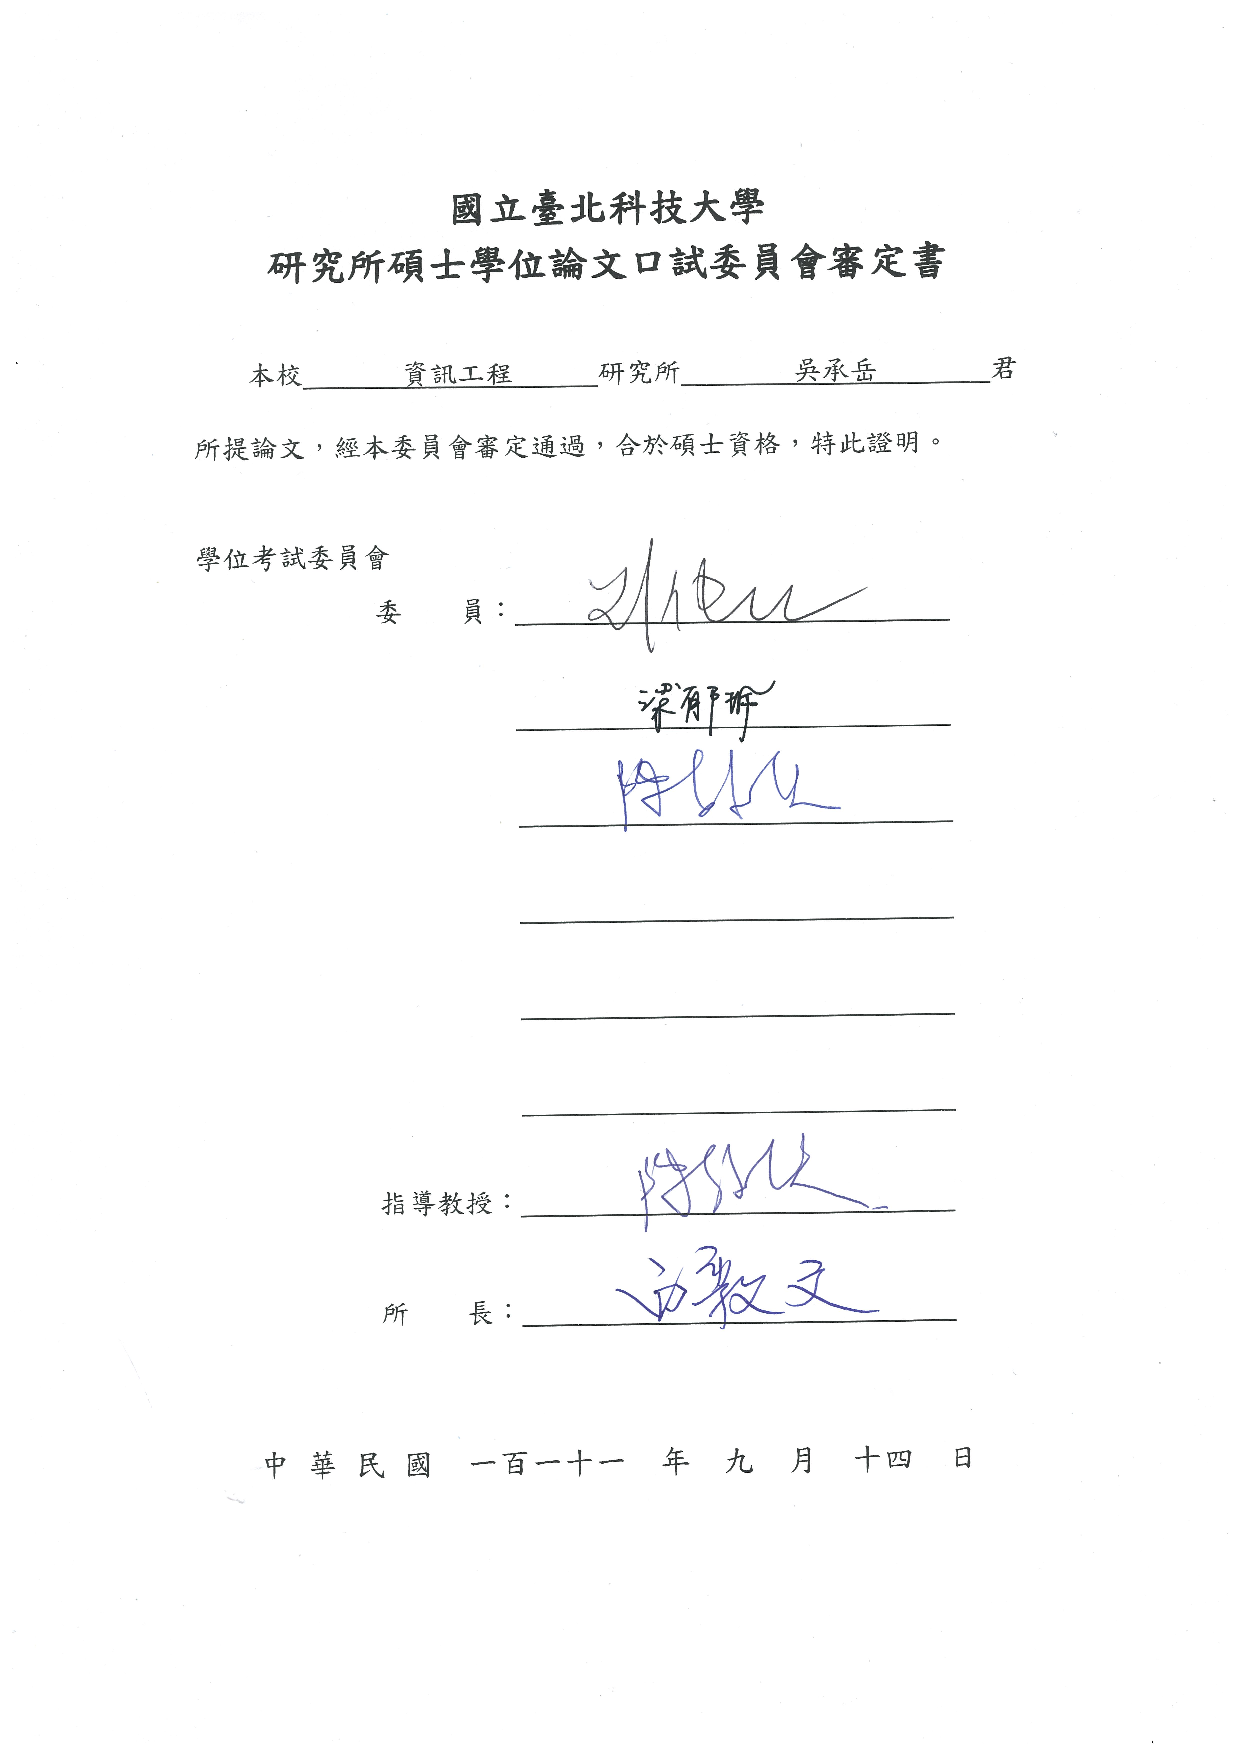
\includepdf[pages={1}]{20220921114815.pdf}

\AddToShipoutPicture{\WatermarkPicture}                     % 加入浮水印

\pagenumbering{roman} 										%論文篇前之頁數為羅馬數字
\chapter*{摘~~要}
\addcontentsline{toc}{chapter}{中文摘要}

%基本資訊

\noindent
論文名稱:以資料冷熱分群之策略增進開放通道固態硬碟空間回收效率 \\%Robot Framework測試腳本重構工具的改善:增加重構方法之多元選擇\\
頁數:29\\
校所別:臺北科技大學~資訊工程系碩士班\\
畢業時間:一百一十學年度第二學期\\
學位:碩士\\
研究生:吳承岳\\
指導教授:陳碩漢 博士\\
%\hspace*{\fill}\\
\noindent
關鍵字:LightNVM、Open-Channel SSD、SSD、Garbage Collection、垃圾回收效率、Linux、Kernel Module\\
\hspace*{\fill}\\
%
\indent
Solid State Drive,簡稱 SSD,是一種近年來被廣泛應用在各種電腦之中的儲存裝置,也因不具機械元件等原因,具有存取速度快,較不會因為震動等外力受損等優點,逐漸提升市占率。但隨著廠商想要壓低成本,這種硬碟的限制也變得更為明顯。

一直以來,SSD 都有三個限制,Erase Before Write 跟 Limited Program/Erase Cycles 跟 Asymmertic Program/Erase Unit,而過去都是讓 SSD 之中 的 FTL (Flash Translation Layer) 獨自管理。但是這樣 SSD 並沒有 Host 的資訊,不知道 Host 想要哪些資料;而 Host 也不知道 FTL 的管理狀況,有可能會,也就是雙方並沒有溝通,造成 Host 與 SSD 雙方的資訊落差,進而導致效率下降。而 Open Channel SSD 就是為了讓 Host 與 FTL 溝通而改良而成的一種新型 SSD。
%針對原本在 Linux 核心中既有的 SSD 管理系統模組 LightNVM,本論文加入一種機器學習演算法,除了保有原先所提供的管理Open Channle SSD之功能,包含管理讀取、寫入、Garbage Collection等功能,我們在寫入之中加入將資料依據特性分類,將經常更改的熱門資料 (Hot data)放在一起,以及將經過許久才修改一次的冷門資料(Cold Data)擺在一起,讓這個模組在做 Garbage Collection 時可以容易將資料一併整理。

\indent
而本論文針對 Open-Channel SSD 提出一個設計方案,將資料劃分為冷門到熱門四個不同的等級,並將資料依照等級分開擺放來增進 Garbage Collection 的效率,。讓 Open-Channel SSD 不再只能循序寫入,現在可以透過集中熱門資料 (Hot Data) 以及冷門資料 (Cold Data),來提升整體效率。最後在寫入相同資料量的狀況下,比較 Garbage Collection 的次數,以驗證是否有提升效率。
%而本論文針對 Open Channel SSD 提出了利用強化學習來增進效率,並選擇 Q-Learning 作為案例分析,其特殊的結構 Q-Table,可將資料劃分等級,紀錄每次寫入時獲得的獎勵 (reward);每次寫入都會用之前紀錄的獎勵值來推測寫在哪個位置的狀況會比較好,以決定當下寫入的位置。讓 Open Channle SSD 不再只能循序寫入,現在可以透過集中 Hot Data 以及 Cold Data,來提升整體效率。


%而這個演算法是一種機器學習演算法 Q-Learning,運用其特殊的結構 Q-Table,將資料劃分等級,紀錄每次寫入時獲得的獎勵 (reward);每次要寫入時,就會用之前紀錄的獎勵值來推測寫在哪個位置的狀況會比較好,以決定當下寫入的位置。讓 LightNVM 所管理的 Open Channle SSD 不再只能循序寫入,現在可以透過集中 Hot Data 以及 Cold Data,來提升整體效率。


%針對本實驗室開發的一個Robot Framework測試腳本重構工具RF Refactoring,本論文提出兩種功能延伸,除了保有原先所提供的三種重構功能,重新命名關鍵字、重新命名變數及修改關鍵字介面之外,新增了抽取重複步驟成為新關鍵字、移動關鍵字宣告的功能,其能夠使工具更加完備,讓開發人員進行相關重構時,不再只能利用搜尋取代的方式進行重構,且不需進行不必要的人工檢查,進而提升重構效率,而在重構方法的選擇上也更加多元。


%\indent
%Robot Framework是一種利用關鍵字驅動的自動化驗收測試框架,其擁有良好的可讀性以及擴充性,因此許多專案都會使用Robot Framework開發自動化驗收測試。當專案到達一定的規模大小,並且團隊有既定的程式碼風格時,測試團隊常會遭遇需要重構關鍵字及測試腳本的問題,例如修改關鍵字名稱、抽取重複步驟等等。過去團隊所使用之重構工具提供了三種重構功能,重新命名關鍵字、重新命名變數、修改關鍵字介面,其幫助測試團隊在進行重構時,不再只能利用搜尋取代的方式進行重構,且不需進行不必要的人工檢查,進而提升重構效率。但目前其重構功能仍然是不足的,測試團隊在進行其他類型的重構時,仍須使用目前用來撰寫Robot Framework測試腳本的整合式開發環境(RED、Visual Studio Code)中的搜尋取代工具進行重構,因而造成重構效率的降低,以及人工檢查的疏忽,導致重構的錯誤和缺漏等等。
%
%\indent
%本論文將為團隊使用中的重構工具增加不同的重構功能,使測試團隊在選擇重構方法時,能夠更加多元,而在重構過程中,也能夠省去多餘的人工檢查,避免搜尋的缺漏及取代的錯誤。										%中文摘要
\chapter*{ABSTRACT}
\addcontentsline{toc}{chapter}{ABSTRACT}

%基本資訊

\noindent
Title:Exploring Hot/Cold Data Separation for Garbage Collection Efficiency Enhancement on Open-Channel SSD\\
Pages:24\\
School: National Taipei University of Technology\\
Department: Computer Science and Information Engineering\\
Time: September,2022\\
Degree: Master\\
Researcher: CHENG-YUEH WU\\
Advisor: SHOU-HAN CHEN, Ph.D.\\
%\hspace*{\fill}\\
Keywords: LightNVM, Open-Channel SSD, SSD, Garbage Collection, Performance, Linux, Kernel Module\\
%\hspace*{\fill}\\
\indent
In the past, the FTL (Flash Translation Layer) in the SSD (Solid State Drive) has been left to manage the SSD internal alone. However, the SSD did not communicate with the Host, resulting in a gap in information between the Host and the SSD, which in turn led to a decrease in efficiency. Open Channel SSD is a new type of SSD that is improved to allow the Host to communicate with the FTL.

\indent
This thesis proposes a method by dividing the data into four different levels, from cold to hot, for Open Channel SSD. We separate the data according to the level to improve the efficiency of Garbage Collection. Open-Channel SSD can no longer only write sequentially. They are able to improve the overall efficiency by centralizing Hot Data and Cold Data now.

%過去都是讓 SSD 之中 的 FTL 獨自管理內部。但是這樣 SSD 並沒有跟 Host 溝通,造成 Host 與 SSD 雙方的資訊落差,進而導致效率下降。而 Open Channel SSD 就是為了讓 Host 與 FTL 溝通而改良而成的一種新型 SSD。 DeepL 翻譯再改的

%This thesis proposes two extensions to RF Refactoring, a Robot Framework test script refactoring tool developed in our laboratory. In addition to the three original features - renaming keyword, renaming variable, and modifying keyword interface - two new features have been added: extracting duplicate steps to a new keyword and relocating keyword definition. With the added features, RF Refactoring is better able to enable developers to carry out relevant refactoring without resorting to search, replace, and manual inspection, thereby improving the efficiency of refactoring.										%英文摘要
\chapter*{誌~謝~}
\addcontentsline{toc}{chapter}{誌謝}

\indent
在此要先感謝我的指導教授陳碩漢老師,由於本身有先離開學校一兩年再回歸學習的環境,雖然大學畢業就是資訊工程系,但是除了為了考試所準備的東西比較熟悉,其他範圍其實已經有點生疏。不過在碩士兩年時光,修了很多作業很多的課程,還有老師的要求不斷的激勵我,讓我在短時間內學習到眾多的專業知識與技能,也讓我有機會鑽研 Linux Kernel,並且包容我的魯莽以及失誤。雖然這段時間有時候也會不知所措,不過最後看到成果,心中還是充滿著喜悅。
\\ \hspace*{\fill} \\
\indent
同時感謝口試委員陳碩漢老師、梁郁珮老師、劉傳銘老師,對於我的論文提出十分多的建議,讓我的論文能夠更加完整。也感謝吳俊青學長和林稟宸學長,在我開始就讀碩士之後,對於我進修課程以及程式設計上給予許多建議。此外也感謝黃國豪同學,在我在寫作業或是研究時如果有想法卡關之類的狀況,都會給予我協助與建議。
此外十分感謝研究室內的同學們、學長們、學弟妹們,在我寫論文的過程中給予我很多幫助,以及兩年內所有的陪伴,在這個環境下成長是一件十分快樂的事情。
\\ \hspace*{\fill} \\
\indent
最後感謝我的家人們對於我在讀研究所時,給予關心以及關懷,讓我可以無後顧之憂準備論文,真的非常感謝你們的支持與鼓勵,讓我知道我不是一個人在面對這一切,並且順利取得碩士學位。
% \indent
%  首先要感謝我的指導教授陳碩漢老師,在這兩年內辛苦的指導,讓我在這些時間內學習到眾多的專業知識與技能,並且讓我有機會擁有一個大型軟體專案開發的經驗,也十分感謝口試委員劉立頌老師、陳碩漢老師,對於我的論文提出十分多的建議,讓我的論文能夠更加完整並且對於研究室內的團隊有所貢獻。

% \indent
%  此外十分感謝研究室內的同學們、學長們、學弟妹們,在我寫論文的過程中給予我很多幫助,並且協助我完成論文所需的實驗,以及兩年內所有的陪伴,有你們在的研究室永遠是最愉快的。

% \indent
%  最後感謝我的家人們對於我在台北讀研究所時,不斷的關心以及關懷,真的非常感謝你們的支持與關心,還有我的女友安安,在我忙碌的時候耐心的陪伴我、鼓勵我,讓我知道我不是一個人在面對這一切,並且順利取得碩士學位。											%誌謝
\newpage


\addcontentsline{toc}{chapter}{目錄}
\tableofcontents 											%引入目錄
\newpage

\addcontentsline{toc}{chapter}{表目錄}
\renewcommand{\numberline}[1]{\lotlabel~#1\hspace*{1em}}
\listoftables												%引入表目錄
\newpage

\addcontentsline{toc}{chapter}{圖目錄}
\renewcommand{\numberline}[1]{\loflabel~#1\hspace*{1em}}
\listoffigures												%引入圖目錄
\newpage													%換新頁

% \addcontentsline{toc}{chapter}{程式碼目錄}
% \renewcommand{\numberline}[1]{\loclabel~#1\hspace*{1em}}
% \lstlistoflistings
% \newpage

\pagenumbering{arabic}										%論文內文之頁數為阿拉伯數字

\chapter{緒論}
\section{研究背景與動機}
\indent
%隨著整個市場對於 SSD 的需求日漸增加,現今的技術也越朝著把更多的資料塞進 SSD 裡面。也意味著對於容量的需求急速成長。
但是SSD的諸多缺點也因此而越來越明顯,寫越多的資料進去,每單位的壽命就越少,資料錯誤的可能性也越高。
也就需要越來越多的技術來維護 SSD 的壽命以及資料的正確性

而 Open Channel SSD 就是在這樣的需求下誕生了,這項技術嘗試把某些以往給 SSD 控制器管理的技術交給 Host 管理,既可以減輕 SSD 控制器的負擔,還能讓 Host 管理哪些是可能之後還會用到的資料,進而只將這些資料存在記憶體,達到減少記憶體使用量及提升快取效率的目的。

而資料通常可能會分為兩種,一種是 hot data,通常很快就會被覆寫,例如暫存檔或是存在硬碟的虛擬記憶體;另外一種是 cold data,會存放很久才有可能會更改,例如照片,影片,遊戲檔案之類的。
現行的 Open Channel SSD 沒考慮到資料特性,目前是以循序寫入為主,這樣極有可能將 Hot Data 及 Cold Data 擺在一起,導致之後後要整理資料時需要花費較多的資源來運作。

相較於SSD controller,host 的資源很豐富有很多 memory 以及強大 CPU,於是我們把強化學習放進去,希望可以透過強化學習,自動化調整資料分配的方式將 Hot Data 以及 Cold Data 分開,進而改善效能。

%\section{研究背景與動機}
%\indent
%Robot Framework\cite{robotframework}是一個自動化測試框架,其中的關鍵字可被視為一個測試步驟,透過將多個關鍵字包裹成一個更高層級的關鍵字時,便可將其視為一個測試流程。

%\indent
%當多個團隊一起開發測試腳本時,關鍵字能夠盡量被重複使用是一個常見的目標。而部份情況中我們可以在撰寫測試腳本時就判斷出撰寫的測試步驟是可以被重複使用,因而將其提前包裹成一個新關鍵字,例如當我們在同一個測試腳本中,有多個步驟需要重複使用時,我們便會提前將其抽取成一個關鍵字提供多處使用,這是可以預知的;但大部分的情況中,我們無法預期目前所撰寫的測試步驟是否會被其他測試腳本再次使用,以兩個測試團隊為例:其中一個測試團隊需要以創立一個項目的流程作為測試腳本中的主要步驟,另外一個測試團隊也需要相同的流程做為測試資料的準備,平時撰寫測試腳本時,兩個組別無法隨時互相溝通,只能以現有的情況做為判斷,因此無法透過提前判斷而去抽取成一個關鍵字,或者其中一個團隊剛好發現其他團隊已有撰寫好之流程,直接拿取做使用且當下未立刻進行抽取關鍵字之重構,導致後續時常需要對現有的程式碼進行重構。

%\indent
%進行重構時,重複的測試步驟往往都是存在於不同的檔案中,一不小心就會有部分程式碼未修改,直到後續執行時才發現錯誤,這些經常都是人為錯漏所導致的。為了避免以上所提及的錯誤不斷發生,導致測試團隊必須再次花費時間針對缺漏的錯誤進行修正,因此在測試團隊重構時,需要一個能夠避免人為錯漏且更加方便的重構工具。

\section{研究目標}
\indent
Open Channel SSD 是一種與作業系統互相合作的一種SSD\cite{robotframework},而 LightNVM \cite{LIU-Thesis}則是在 Linux 核心模組中專門管理 Open Channel SSD 的模組,此模組目前是以循序寫入的模式實作,不過並沒有將資料分類,再依據各分類改變寫入位置,而我們認為可能還有改善效率的空間,因此本論文將針對此模組修改以增進效能。
\indent
首先我們將資料分為熱門資料 (Hot Data) 以及冷門資料 (Cold Data),再用 Q-Learning 演算法計算每次寫入動作的獎勵值 (reward),而每次寫入時參考之前紀錄的這些獎勵值,決定將這次的要求寫入到最佳的位置,以達到最佳的效率。

%\section{研究目標}
%\indent
%劉冠志論文\cite{LIU-Thesis}中提供了測試腳本重構工具RF Refactoring,此工具提供了三種Robot Framework測試腳本的重構方法,分別為重新命名關鍵字、重新命名變數,以及修改關鍵字介面,但仍然無法解決目前所遭遇之問題,因此本論文將針對此工具進行改善,否則開發人員只能使用目前用來撰寫Robot Framework測試腳本的整合式開發環境(RED\cite{RED}、Visual Studio Code\cite{VSCode})中的搜尋取代工具進行重構,因而造成重構效率的降低,以及人工檢查的疏忽,導致重構的錯誤和缺漏等等。為此工具增加重構方法之多元選擇,使其可根據測試人員的需求重構測試腳本,並且在重構過程中能夠避免人為錯漏的問題發生。

\section{論文組織架構}
\indent
本論文共有六章節,第二章將介紹背景知識及使用工具,第三章介紹 Q-Learning 演算法之方法設計,其中介紹了欲修改的 LightNVM 模組運作模式,並且介紹如何將 Q-Learning 加入至 LightNVM 模組中,第四章將會以第三章所設計之方法進行實作,其中包含了 Q-Learning、Q-Table,第五章將以實際效能測試工具測試讀寫效能,並且與原本無修改的 LightNVM 比較,後續分析實踐結果之差異。

%本論文共有六章節,第二章將介紹背景知識及使用工具,第三章介紹擴充RF Refactoring之方法設計,其中介紹了欲擴充之重構方法及其流程,並且介紹如何將重構方法擴充至RF Refactoring中,第四章將會以第三章所設計之方法進行實作,其中包含了重構流程及外掛程式之實作,第五章將以實際Robot Framework測試腳本介紹重構案例,並且邀請測試團隊成員分別使用Visual Studio Code搜尋取代工具及本論文擴充後之重構工具進行重構,後續比較使用之差異。
\chapter{背景知識}

\section{SSD}\label{s2.1}
\indent
SSD,全名:Solid State Drive,中文:固態硬碟。相較於傳統硬碟(HDD),SSD改善了噪音、震動、讀寫速度慢,容易因震動外力等因素而毀損等等的問題;SSD 也不需要在資料分散時,藉由重組硬碟磁區來減少讀取時間。而重點是,SSD作為儲存裝置,還具有這些優點:\cite{SSD}
\begin{itemize}
    \item 存取時間固定,不像 HDD 有不穩定的搜尋時間
    \item 體積較小,適合放在手機、筆記型電腦等行動裝置之中
    \item 少了機械結構,所以不會因機械故障導致毀損
\end{itemize}

而這些都是因為 SSD 採用了 NAND FLASH Memory。

\subsection{NAND FLASH Memory}\label{s2.1.1}
\indent
是電子抹除式可程式化唯讀記憶體(Electrically-Erasable Programmable Read-Only Memory,簡稱EEPROM或E2PROM)的其中一種,通常為 SSD、記憶卡、以及隨身碟的主要材料元件,可透過電子方式多次複寫。\\
這種元件的基本單位為 cell,而依據每個 cell 可儲存的 bit,可分為:
\begin{itemize}
    \item \textbf{SLC:}Single-level cell   一個 cell 存一個位元
    \item \textbf{MLC:}Multi-level cell    一個 cell 存兩個位元
    \item \textbf{TLC:}Triple-level cell   一個 cell 存三個位元
    \item \textbf{QLC:}Quad-level cell     一個 cell 存四個位元
\end{itemize}
不過,所有的 NAND FLASH Memory均具有以下特性:
\begin{itemize}
    \item Asymmertic Program/Erase unit
    \item Erase before write
    \item Limited P/E cycles
\end{itemize}
以下將一一介紹這些特性。

\subsection{Asymmertic Program/Erase unit}\label{s2.1.2}
\indent
Flash cell 會由多個組成一個 page,而數以百計的 page 會組成一個 block。\\
而 Asymmertic Program/Erase unit 指的意思是,當要讀取或是寫入時,可以 page 為單位寫入,但是如果要 erase 的時候,一次只能以 block 為單位,無法以 page 為單位 Write/Read 跟 Erase 的大小不一樣,所以稱為 Asymmertic (非對稱)。
\begin{figure}[H]
    \centering
    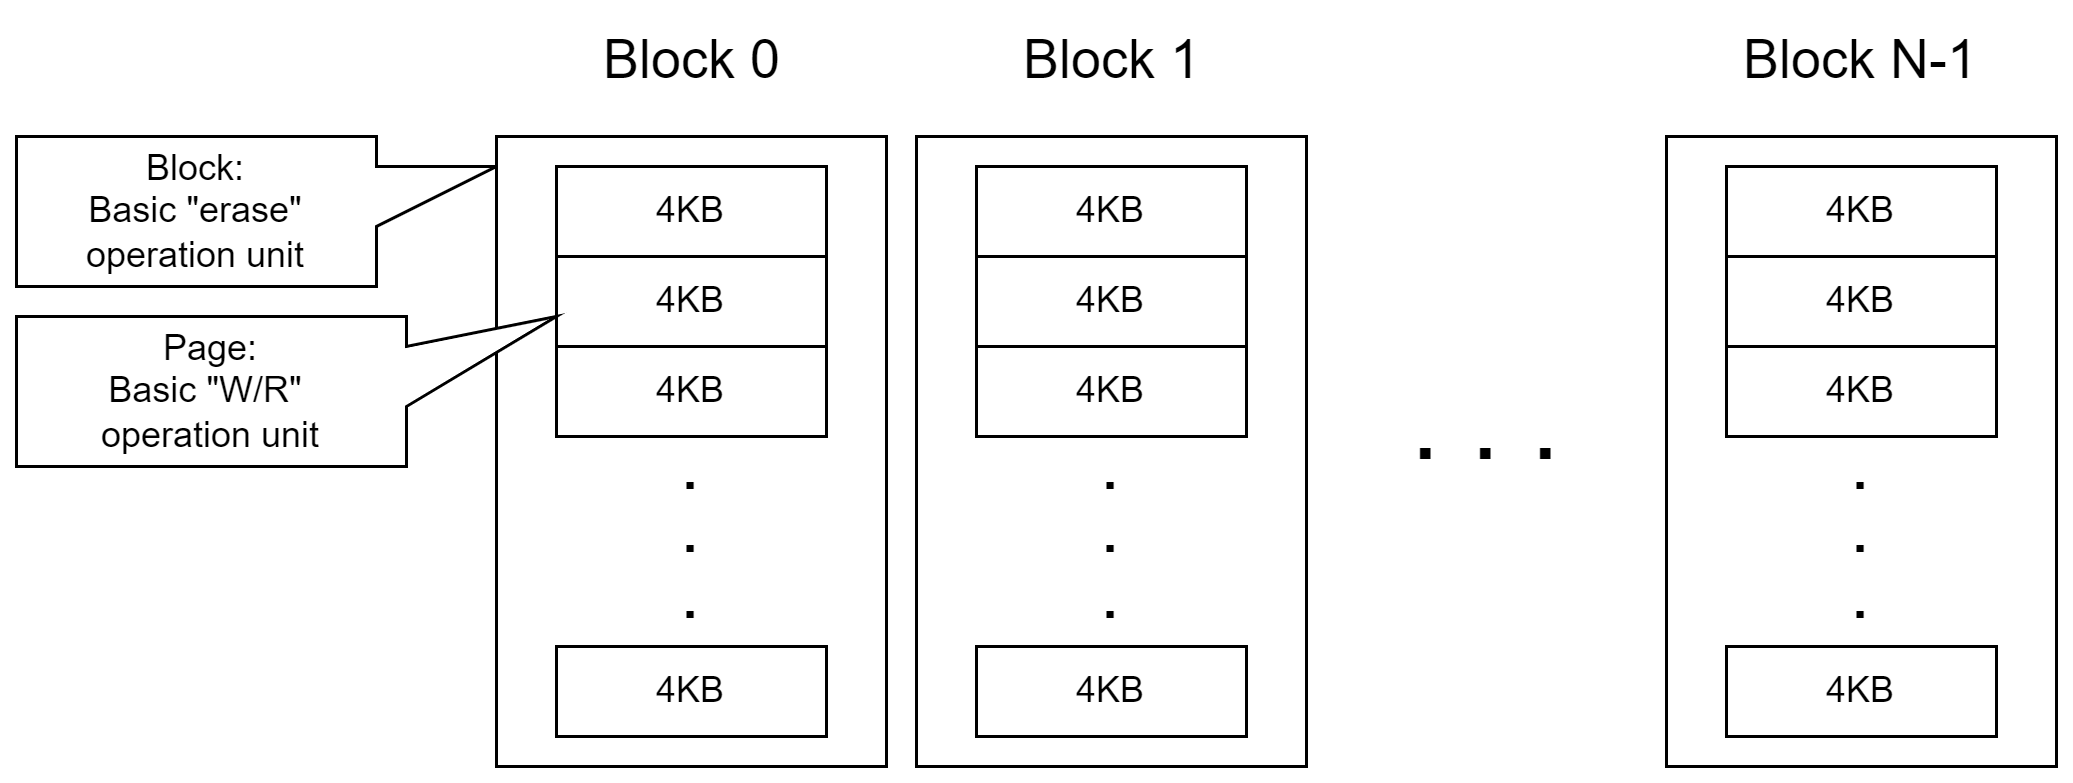
\includegraphics[width=1\textwidth]{picture/ch2/Asymmertic_P-E_unit.png}
    \caption{Asymmertic Program/Erase unit}
    \label{f2.1}
\end{figure}

\subsection{Erase before write}\label{s2.1.3}
\indent
一旦寫入資料到一個 Page 裡面,如果要更改 Page 裡面的資料,只能先清空(Erase),再將資料寫入。而且如\ref{s2.1.2}節所述,清空時還只能清空比 Page 還大的 Block 才行。\cite{SRFTL}
\begin{figure}[H]
    \centering
    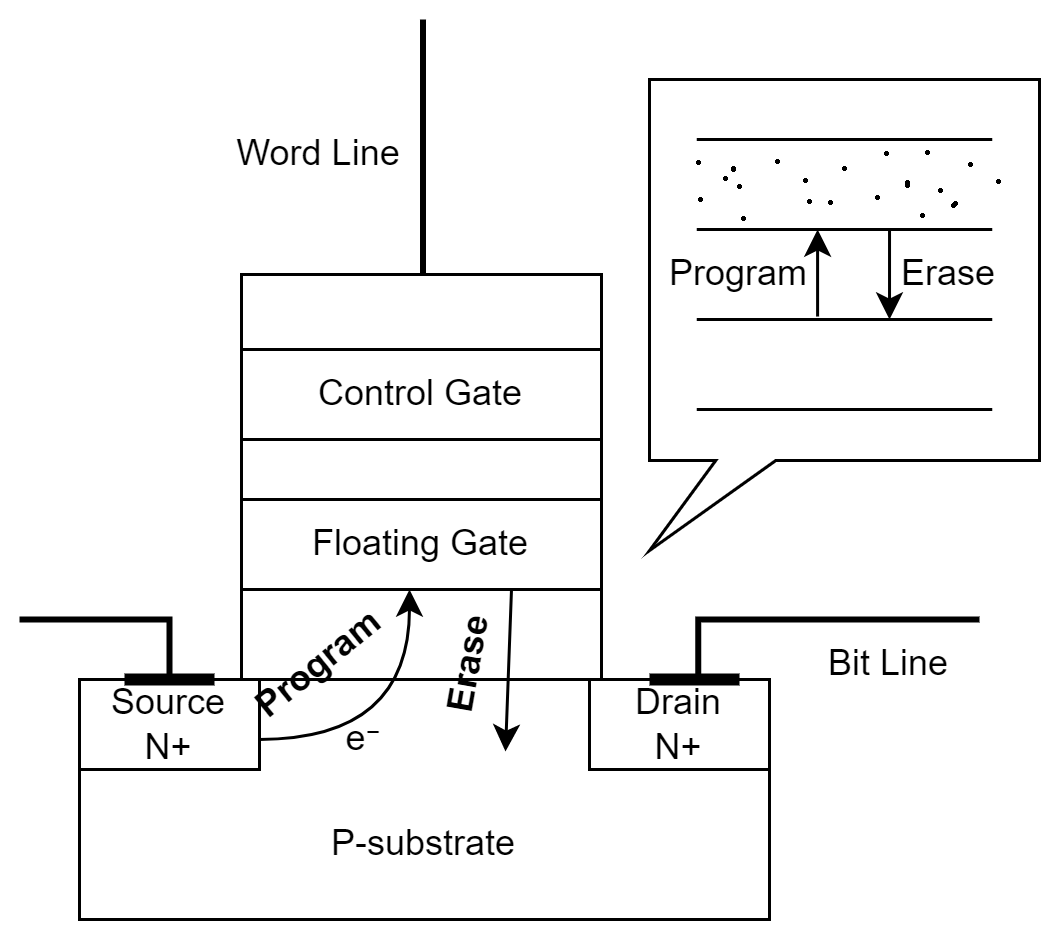
\includegraphics[width=0.6\textwidth]{picture/ch2/erase_before_write.png}
    \caption{Erase before write}
    \label{f2.2}
\end{figure}

\subsection{Limited P/E cycles}\label{s2.1.4}
\indent
Limited Program/Erase Cycle,簡稱Limited P/E cycle,又被稱為 Wear out。重複的寫入會為用來儲存電子的 Flash Memory Cell 帶來不可逆的損害,因為隨著每次電子出入 Cell 的同時,Floating Gate 旁邊的 Oxide layer 就會越來越薄,最後薄到無法鎖住電子,整個 Cell 就會毀損\cite{8631191}。而隨著 Flash Memory 的製造商想要把越多的位元塞進一個 Cell 裡面,這些 Cell 的壽命就越來越少,例如 MLC,TLC,QLC 等等。
\begin{figure}[H]
    \centering
    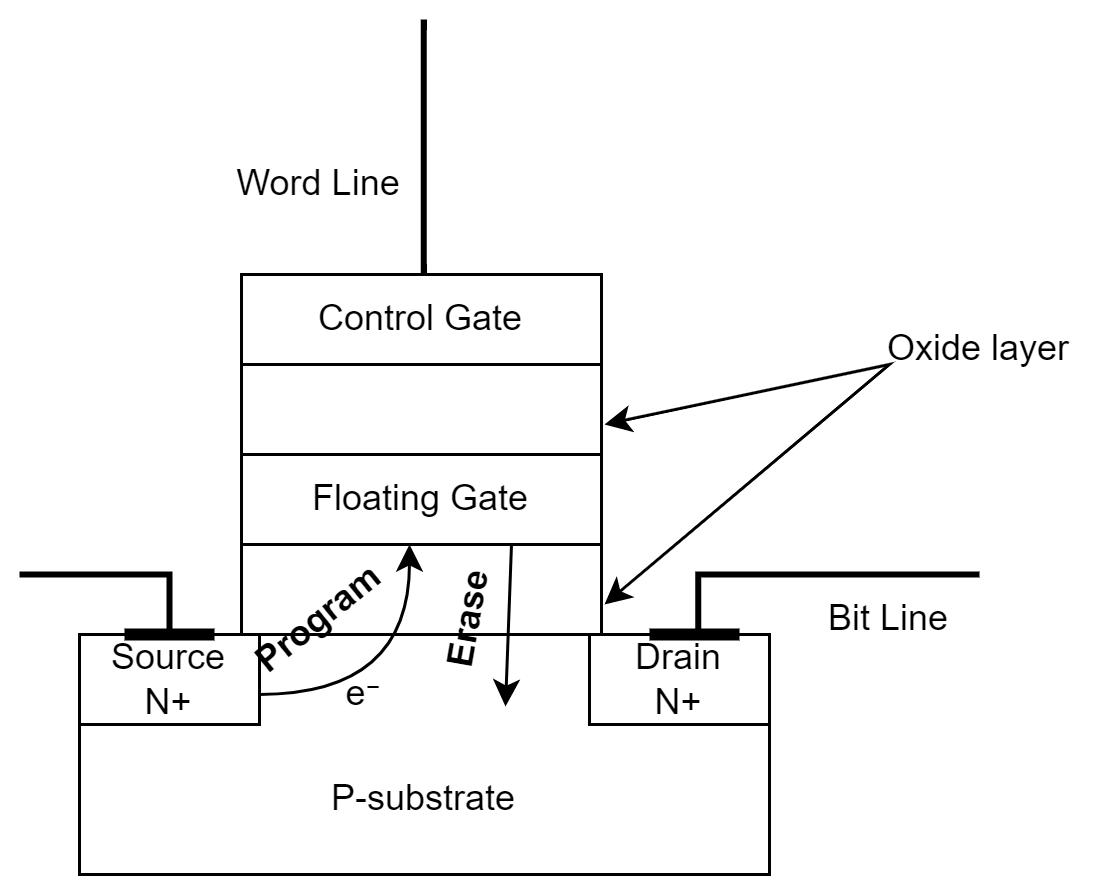
\includegraphics[width=0.6\textwidth]{picture/ch2/Limited_P-E_Cycles.png}
    \caption{Limited P/E cycles}
    \label{f2.3}
\end{figure}

\section{FTL}\label{s2.2}
\indent
為了降低\ref{s2.1.2}節至\ref{s2.1.4}節所提到的特性所造成壽命銳減的問題,SSD的製造商通常都會將 FTL 導入至 SSD 裡面。
FTL 的全名為 Flash Translation Layer,負責管理為了降低 Flash Memory 帶來的錯誤而產生的技術,再模擬成一個普通的硬碟,讓作業系統管理SSD與傳統硬碟 (HDD) 的方式一致。而其中的技術通常包含:\cite{Boukhobza2014ASA}
\begin{itemize}
    \item Wear Leveling
    \item Mapping Table
    \item Garbage Collection
\end{itemize}
\begin{figure}[H]
    \centering
    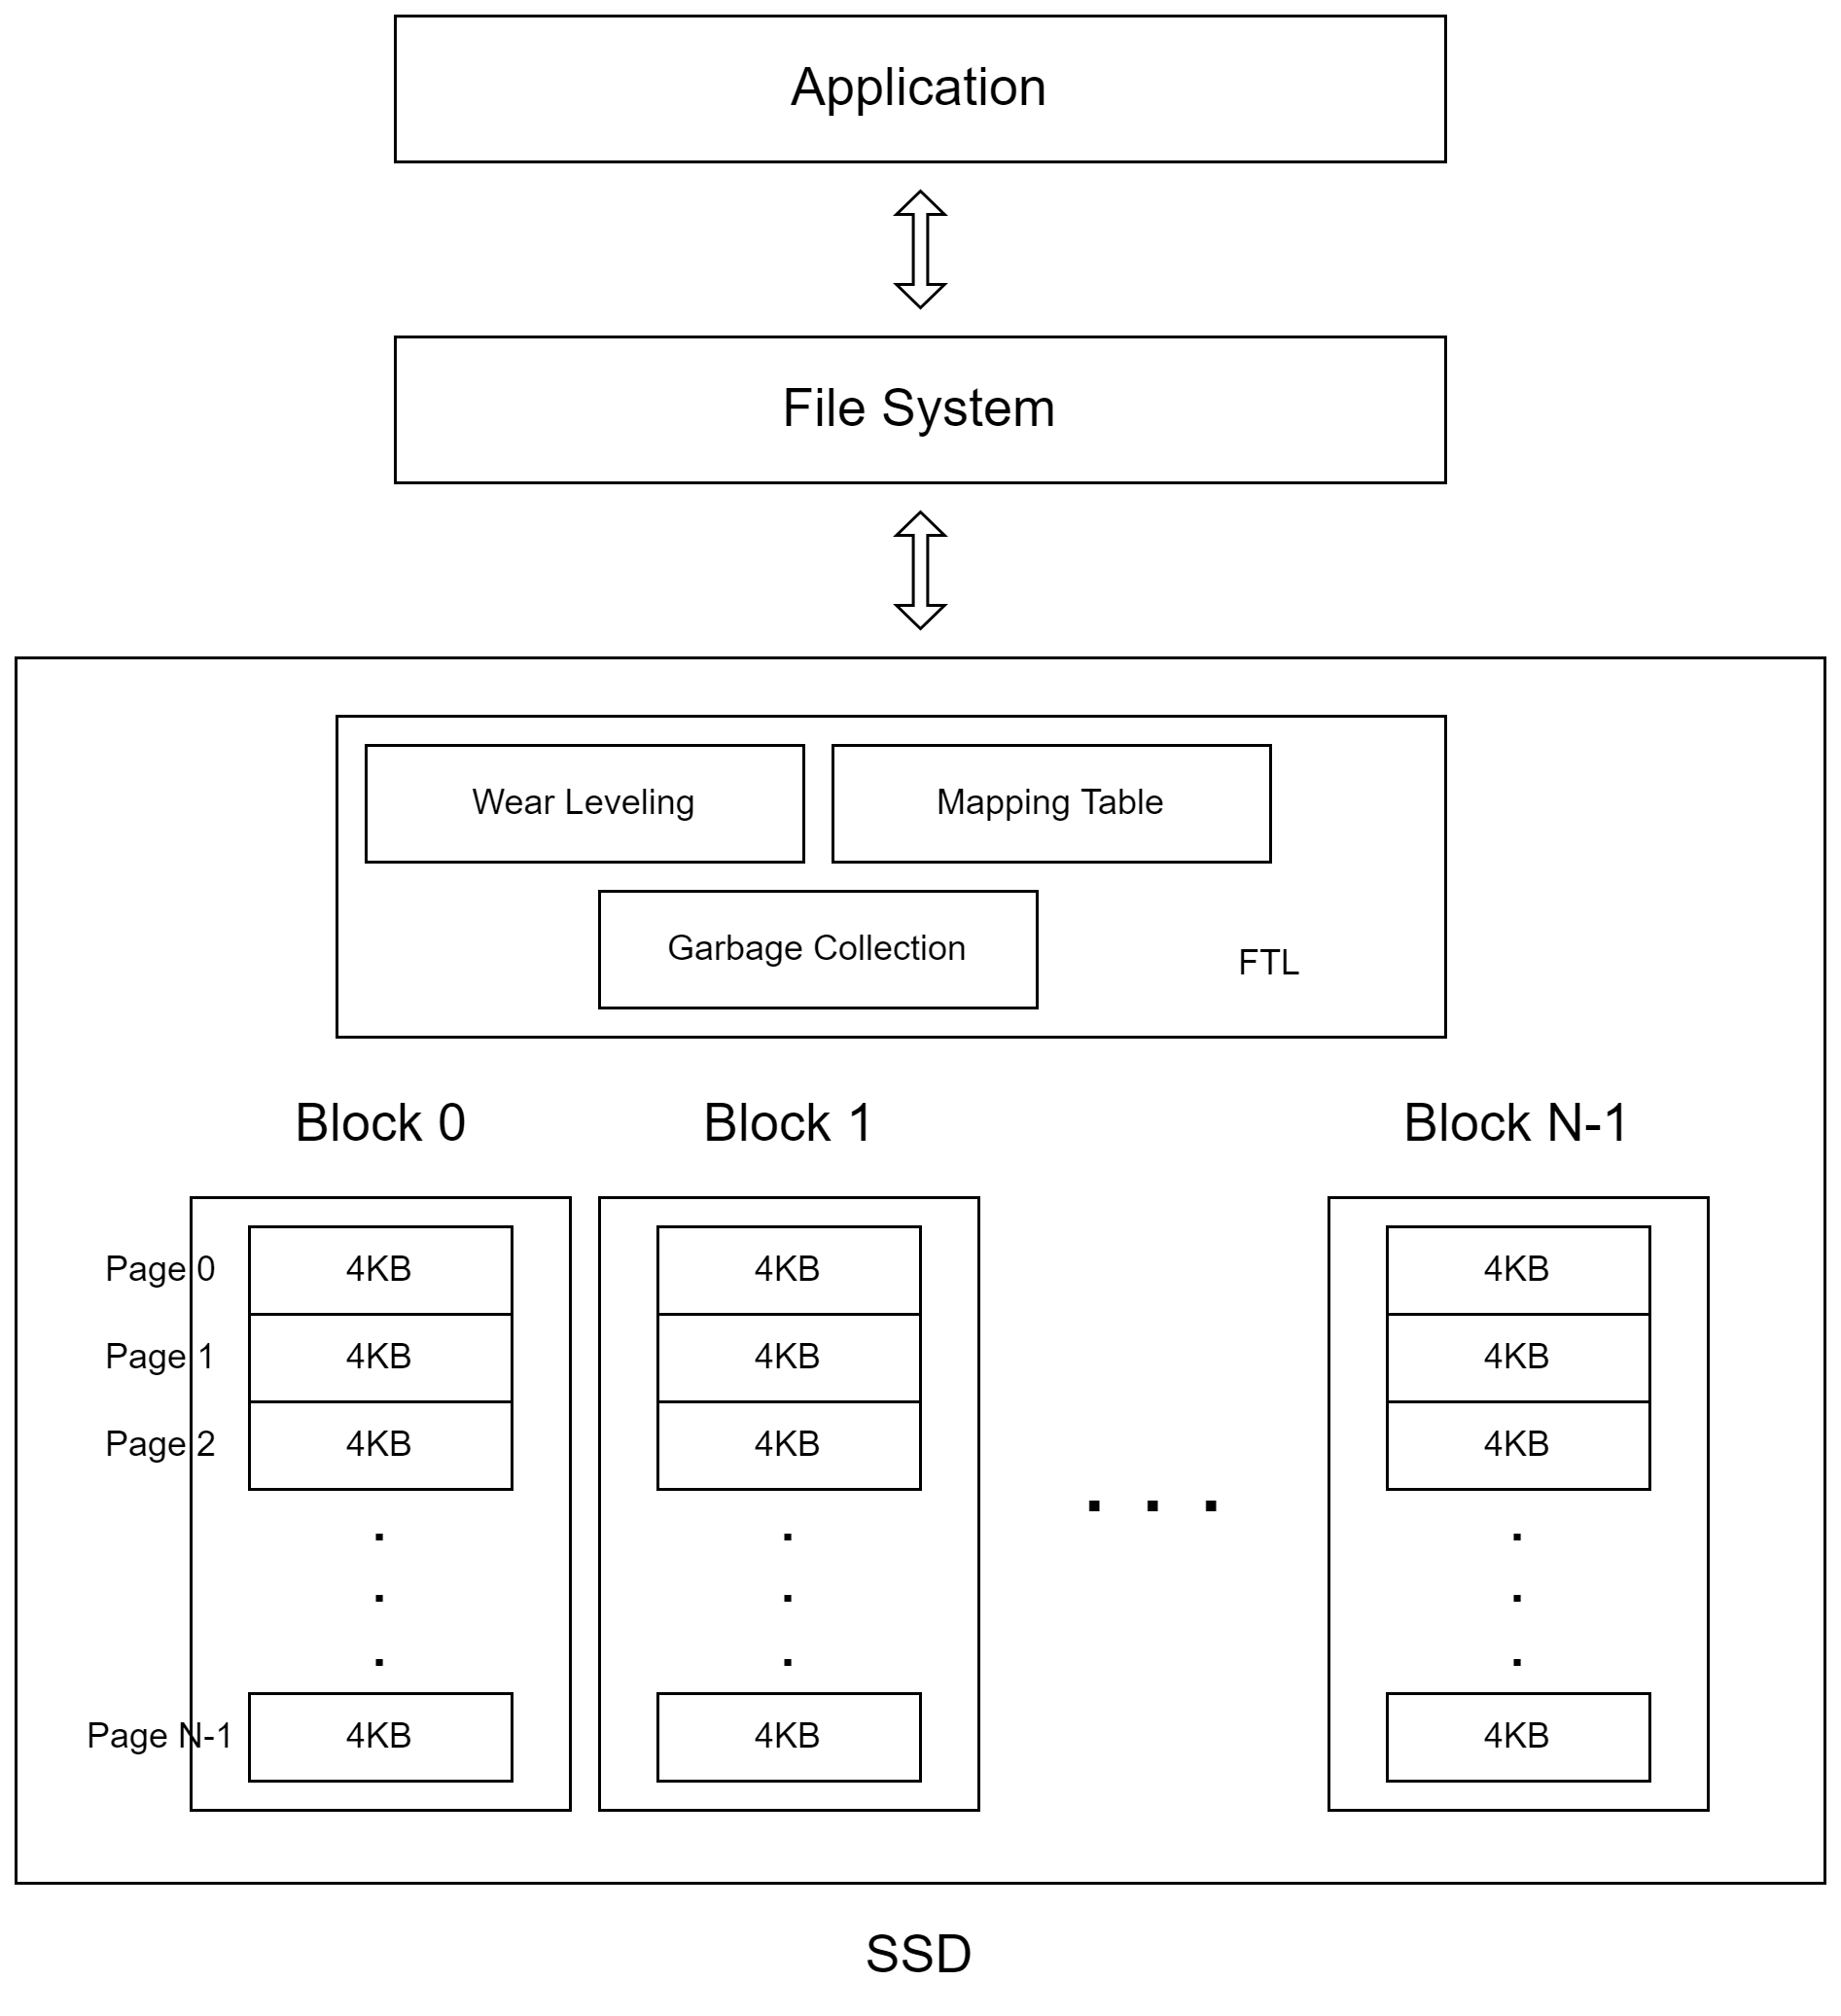
\includegraphics[width=0.7\textwidth]{picture/ch2/FTL.png}
    \caption{Flash Translation Layer}
    \label{f2.4}
\end{figure}
以下將一一介紹這些技術。

\subsection{Wear Leveling}\label{s2.2.1}
\indent
因為\ref{s2.1.4}節所提到的問題,如果每次都寫入同一個位置會導致 Cell 的壽命會銳減,因此為了延長每個 Cell 的壽命,寫入時需要從壽命比較長的 Cell,也就是當下寫入次數較少的 Cell 開始寫入,以平衡整體 SSD 的壽命。所以 SSD 會記錄每個 Cell 的存取次數,來決定下次要寫入到哪裡。\cite{Wear_Leveling_Thesis}
\begin{figure}[H]
    \centering
    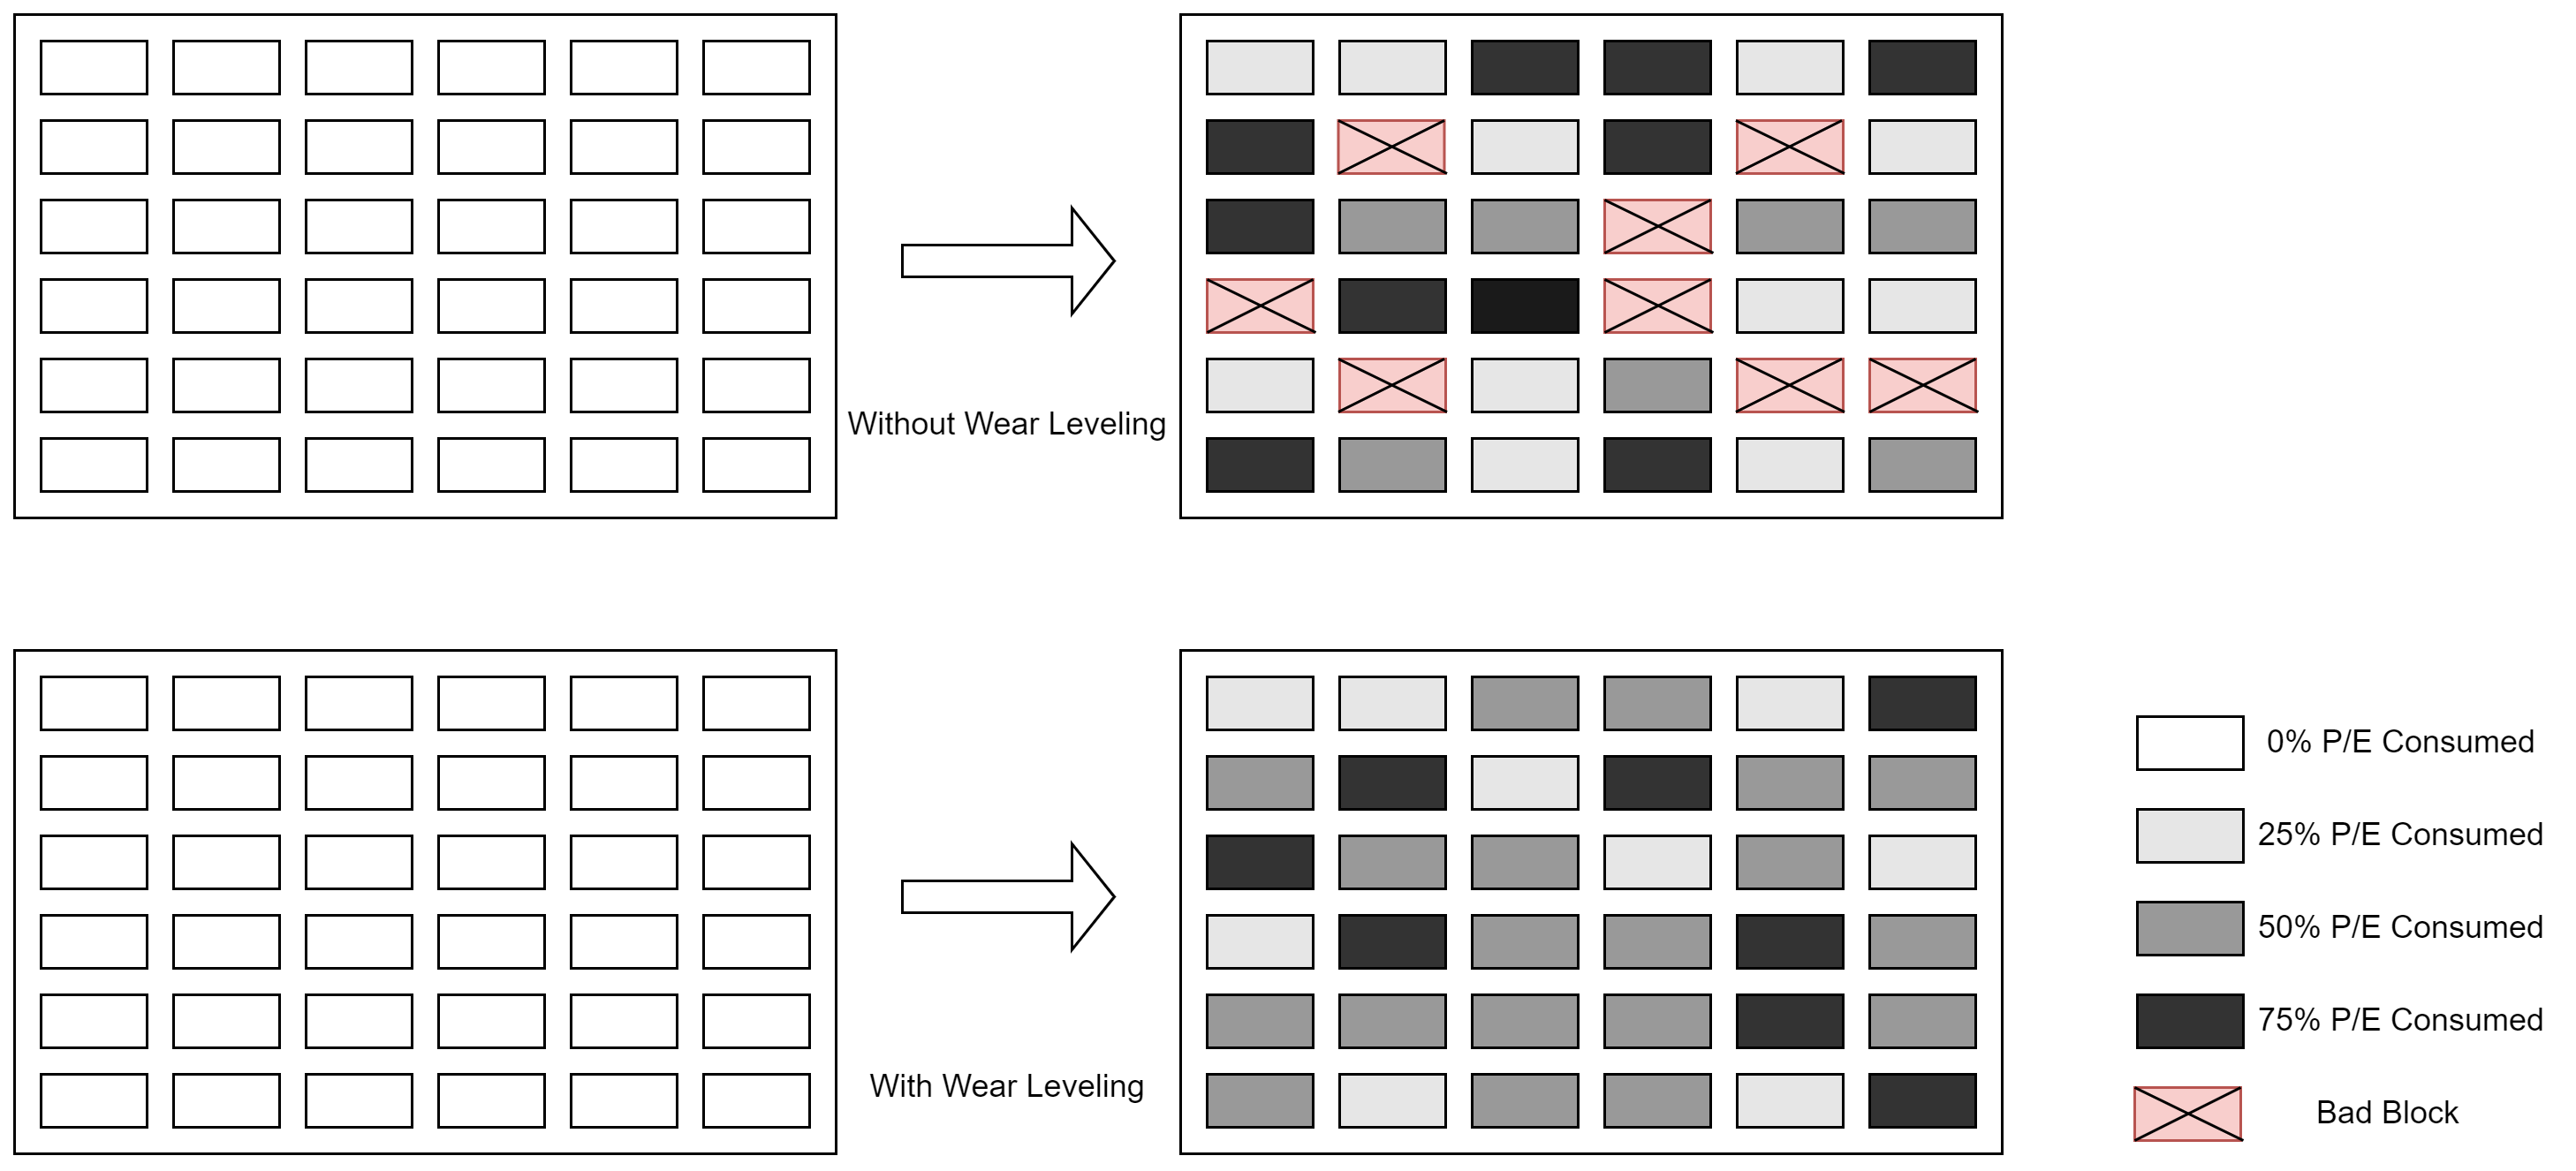
\includegraphics[width=1\textwidth]{picture/ch2/Wear_Leveling.png}
    \caption{Wear Leveling\cite{Wear_Leveling_Pic}}
    \label{f2.5}
\end{figure}

\subsection{Mapping Table}\label{s2.2.2}
\indent
由於\ref{s2.1.3}節所提到的 Erase before Write 問題,因此在 SSD 會先將接到的資料暫存起來,之後寫到其他地方,這樣可以減少寫入的延遲;但同時為了讓 Host 覺得使用跟 SSD 與傳統硬碟的方式一致,就多了一個轉換表,紀錄 Host 傳給SSD的 Logical Address 是對應到實際的哪個Physical Address。通常會跟 \ref{s2.2.1} 所提到的 Wear Leveling 結合。
\begin{figure}[H]
    \centering
    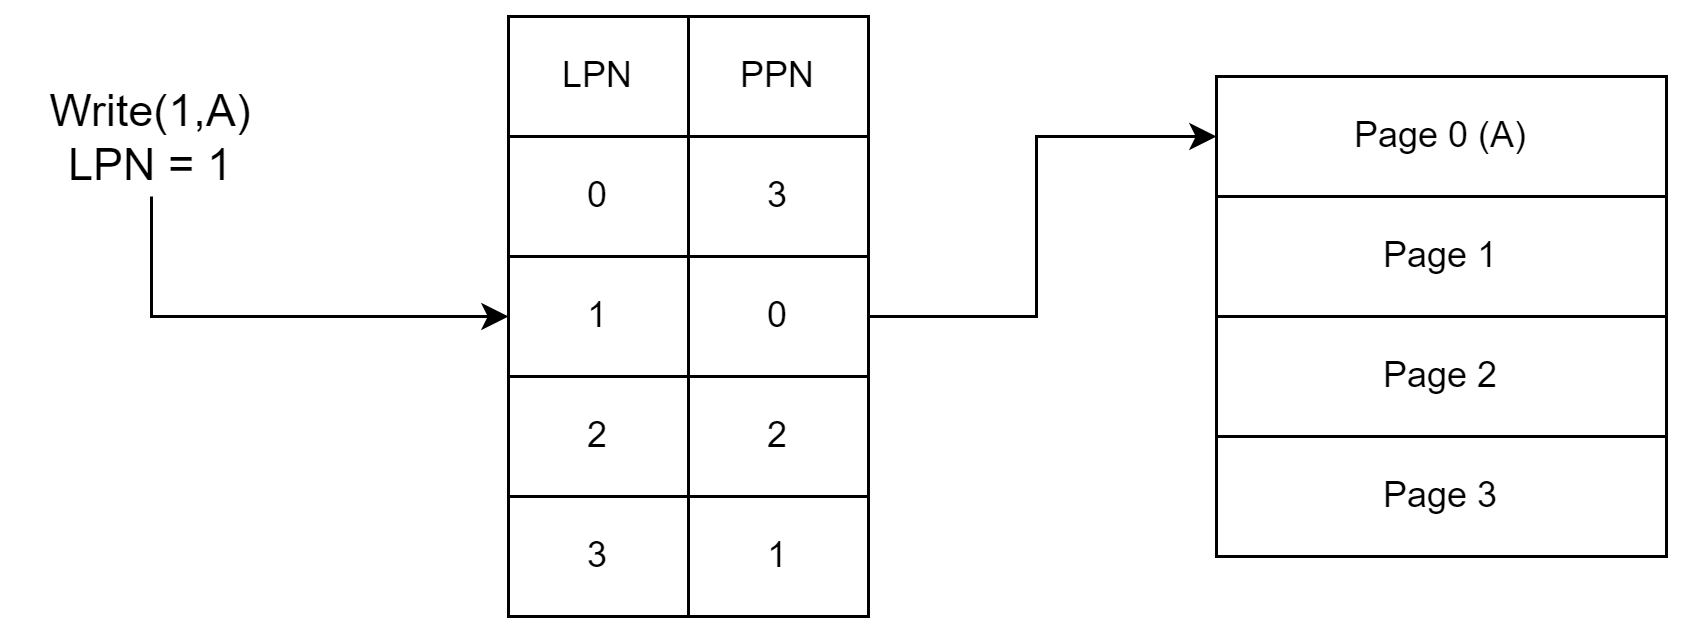
\includegraphics[width=1\textwidth]{picture/ch2/mapping_table.png}
    \caption{Mapping Table\cite{Mapping_Table}}
    \label{f2.6}
\end{figure}

\subsection{Garbage Collection}\label{s2.2.3}
\indent
由於\ref{s2.2.2},將資料寫到別的位置時,原本位置的 block 就會有某些資料被視為無效,但還是有些資料是有效的,這時候就需要讀出來放到其他 block 裡面,才可以將原本位置的 block 清空,繼續當成空的 block 寫入。由於清除資料時的延遲較高,FTL 通常都會挑比較空閒的時候才做這些搬移資料、清空的動作。
\begin{figure}[H]
    \centering
    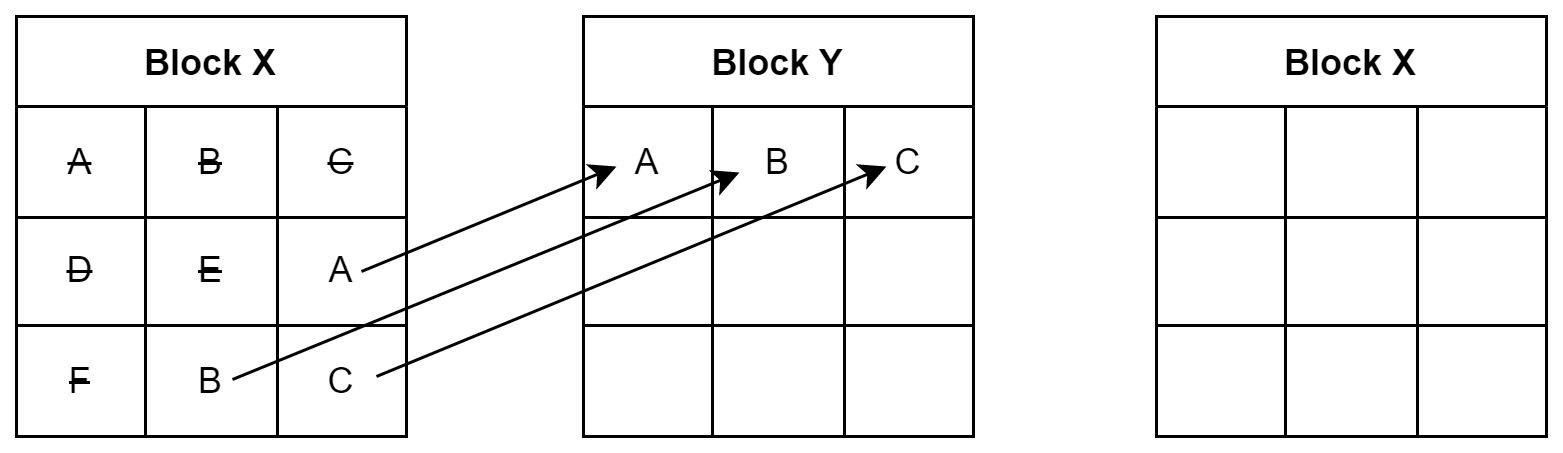
\includegraphics[width=1\textwidth]{picture/ch2/garbage_collection.png}
    \caption{Garbage Collection\cite{Garbage_Collection}}
    \label{f2.7}
\end{figure}

\section{Open Channle SSD}\label{s2.3}
\indent
雖然 SSD 已經有了上述技術來管理以及延長壽命,不過由於這些功能都位於 SSD 內部的 FTL,Host 不知道這些資訊。而在雙方沒有溝通的狀況下,SSD 其實不知道 Host 想要的資料是什麼,容易造成重複讀取或是效率下降的問題,例如 SSD 可能會 caching 到 Host 不需要的資料等問題。
而 Open Channel SSD 開啟了一個可以利用 host 資訊增進存取效能的可能性。
%雖然 SSD 已經有了上述技術來管理以及延長壽命,不過由於這些技術仰賴於 SSD 內部的控制器及韌體管理,Host 完全不知情,所以寫入及讀取的延遲時間取決於韌體以及SSD控制器的穩定度,而為了讓延遲時間能夠掌控在 Host 的手上,也同時為了降低成本,於是有了Open Channel SSD。Open Channle SSD 將下列技術往上交給 Host 管理。
\begin{itemize}
    \item Mapping Table
    \item Garbage Collection
    \item 部分的 Wear Leveling
\end{itemize}
\begin{figure}[H]
    \centering
    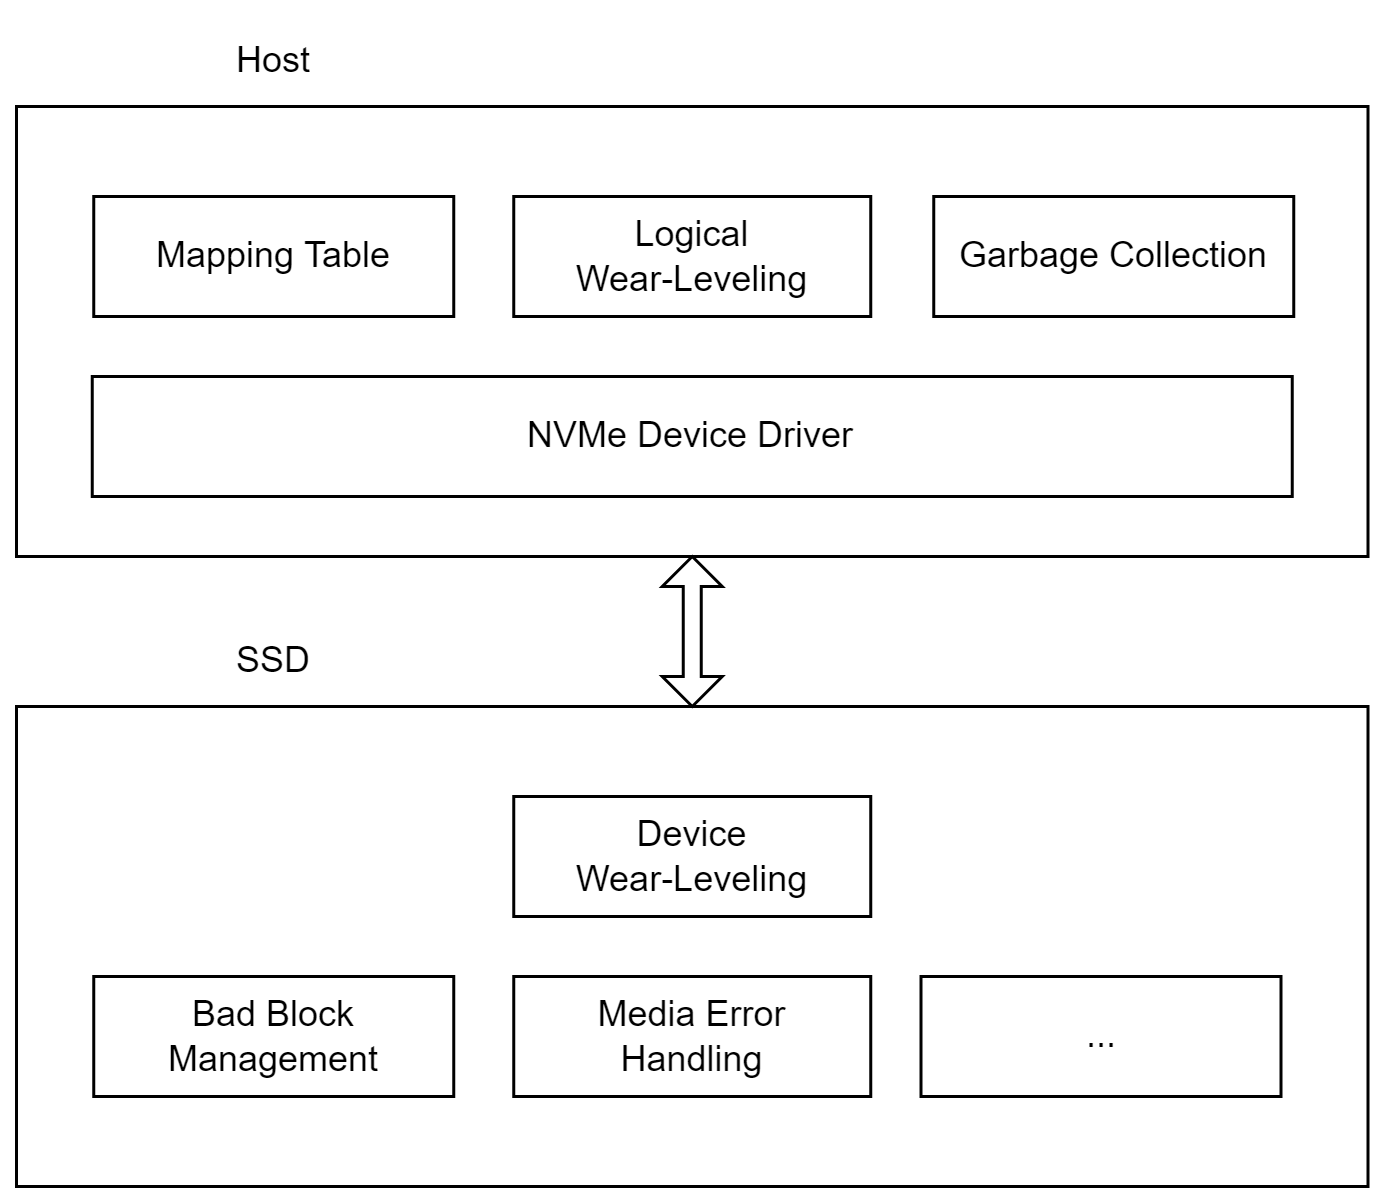
\includegraphics[width=1\textwidth]{picture/ch2/OPSSD.png}
    \caption{Open Channle SSD\cite{OPSSD}}
    \label{f2.8}
\end{figure}

\section{LightNVM}\label{s2.4}
\indent
LightNVM 是 Linux 之中用來管理 Open Channel SSD 的一個 Kernel Module (模組),來實作上述交給 Host 管理的功能,使其可以讓 Linux 系統正確辨識並能夠用控制一般SSD的方式對 Open Channel SSD 提出讀取、寫入、刪除等要求。本論文也是修改此模組來實作我們所需的功能。

\subsection{Line}\label{s2.4.1}
\indent
一般來說,SSD 內部的大小單位可以分為下列幾種,由大而小依序為:
\begin{itemize}
    \item Channel
    \item Lun
    \item Block
    \item Page
    \item Sector
\end{itemize}
而 Line 會由每個 Lun 之中的一個 Block 所組成,如圖2.9所示。而在 LightNVM 之中,寫入以及 Garbage Collection 均採用此單位作為管理的主要架構,本論文提出的修改部分也與此有關。
\begin{figure}[H]
    \centering
    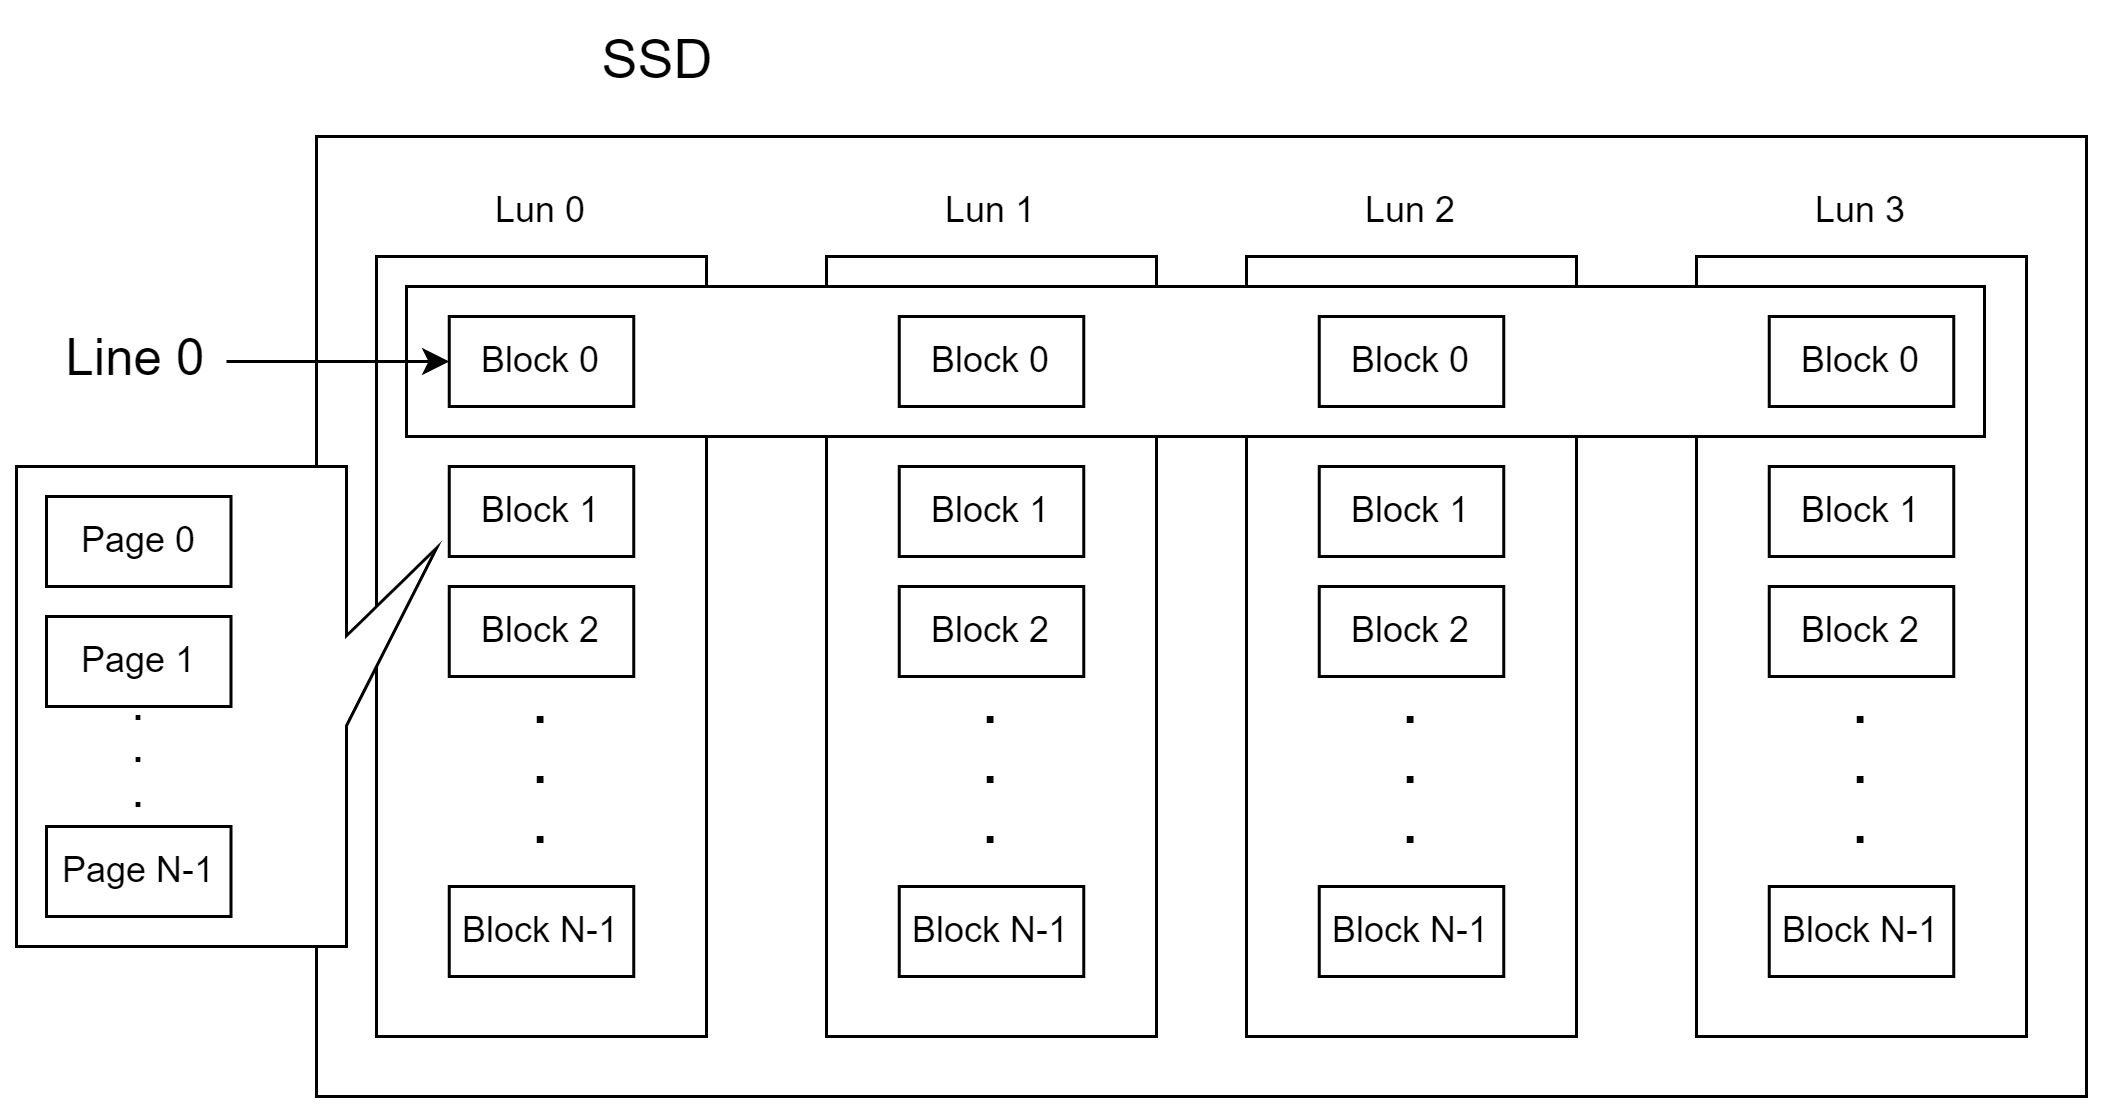
\includegraphics[width=1\textwidth]{picture/ch2/Line.png}
    \caption{單位大小}
    \label{f2.9}
\end{figure}
\chapter{LightNVM 寫入流程之修改設計}
\indent
本論文為提升 Garbage Collection 的效率,以及降低 Garbage Collection 的次數,而提出此設計。透過實作新的演算法,將其與 LightNVM 既有的寫入流程結合,如此一來,LightNVM 在寫入時,會透過這個方法挑選寫入位置,以達成提升效率的目的。\\
\indent
修改大致可分為三部分,第一部分為初始化,讓原本 LightNVM 從準備一個 Line 變成準備四個 Line,一部分為 LightNVM 處理檔案系統的 Request,將資料存入 Ring Buffer;另一部分為 LightNVM 的 Write Thread 會被喚醒,檢查 Ring Buffer 並將 Entry 中紀錄的資料取出,寫到真正的SSD之中,本章節會解釋修改這兩部分的哪些環節。

\section{初始化時修改為準備四個 Line}\label{s3.1}
\indent
在初始化時,LightNVM 會先準備好一個 Line,後續有檔案系統傳遞給 LightNVM 寫入要求時,就會從這個 Line 開始寫入,滿了之後會繼續挑選下一個有空間的 Line 來使用,因此我們為了將資料分開寫入,要修改為在初始化時先準備好四個 Line,以便之後的寫入分群使用。

\begin{figure}[H]
    \centering
    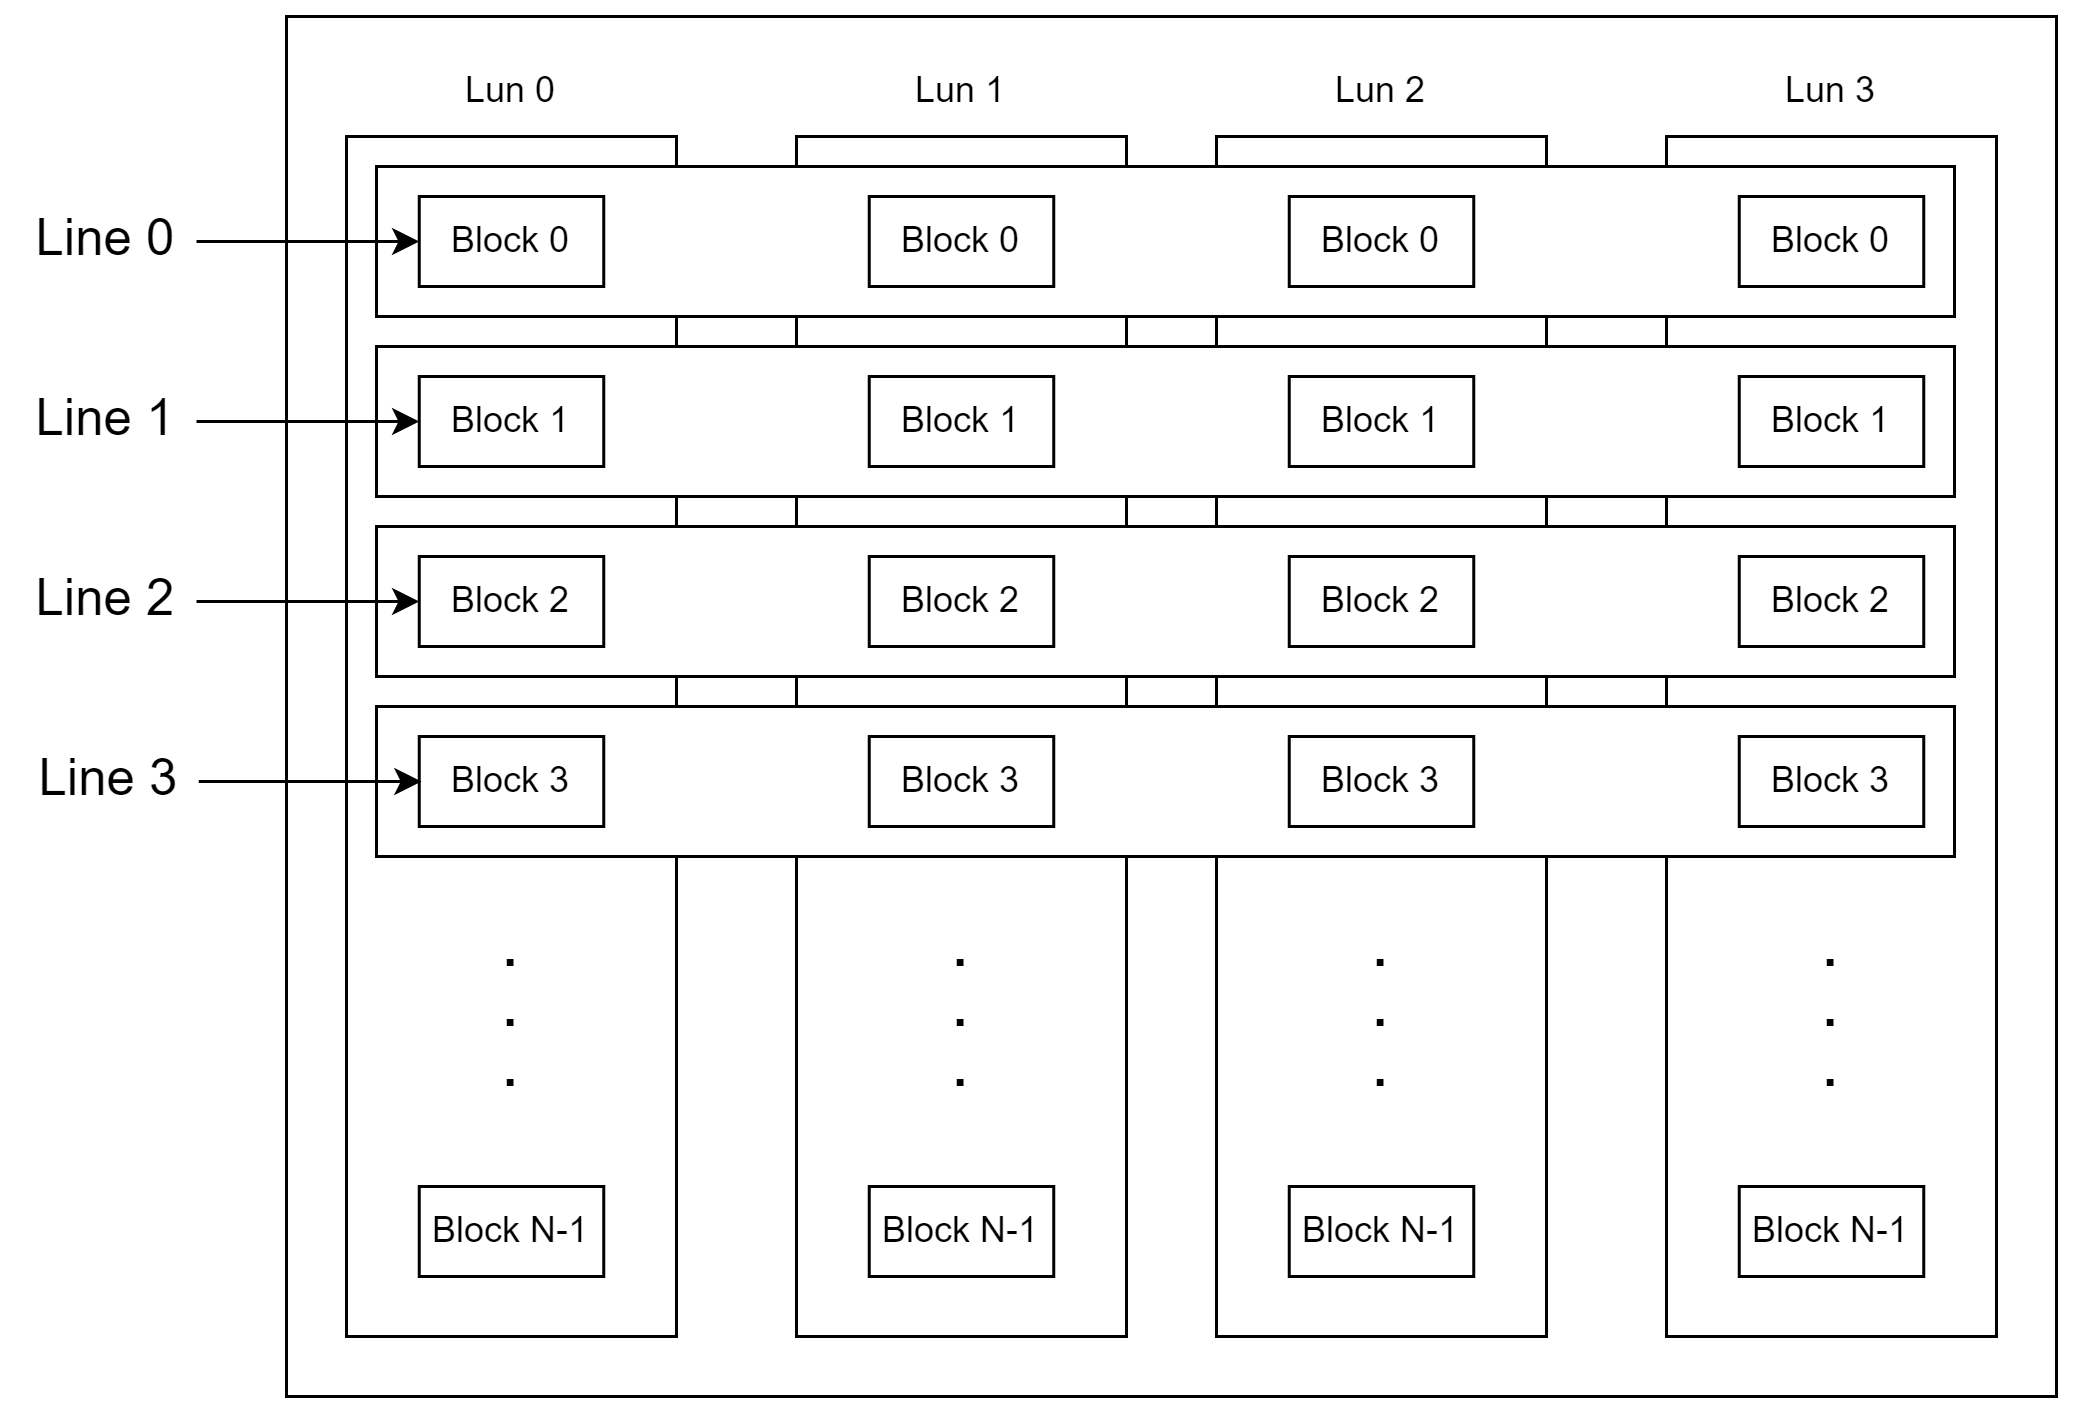
\includegraphics[width=1\textwidth]{picture/ch3/4Line.png}
    \caption{準備四個 Line}
    \label{f3.1}
\end{figure}

\section{處理檔案系統要求之流程}\label{s3.2}
\indent
檔案系統提出 Request 要求之後,LightNVM 會對 Request 拆解,儲存成 LightNVM 自己容易處理的形式,但是在拆解的同時,會損失一些資訊,所以首先我們要先在拆解 Request 之前把 Request 的大小先從 Request 的資料結構 bio (Block I/O) \cite{10.1145/2619092}擷取出來,用大小來判斷這個 Request 的資料屬於哪一個分群,並將資訊塞入 LightNVM 用來儲存 Request 的地方 - Ring Buffer 之中,最後再計算平均值,給下次 Request 傳進時使用。\cite{LightNVM}
\newpage

\subsection{以平均值劃分熱門資料及冷門資料}\label{s3.2.1}
\indent
首先為了劃分熱門以及冷門資料,我們將過去一萬筆 Request 大小的平均值當作基準,劃分四個等級,平均值的 0\% - 50\% 為最熱門的資料,平均值的 50\% - 100 \% 為第二熱門的資料,平均值的 100\% - 150\% 為第二冷門資料,平均值的 150\% 以上為最冷門的資料。並且由熱門到冷門,我們會分配到 Line 0 到 Line 3。
\begin{figure}[H]
    \centering
    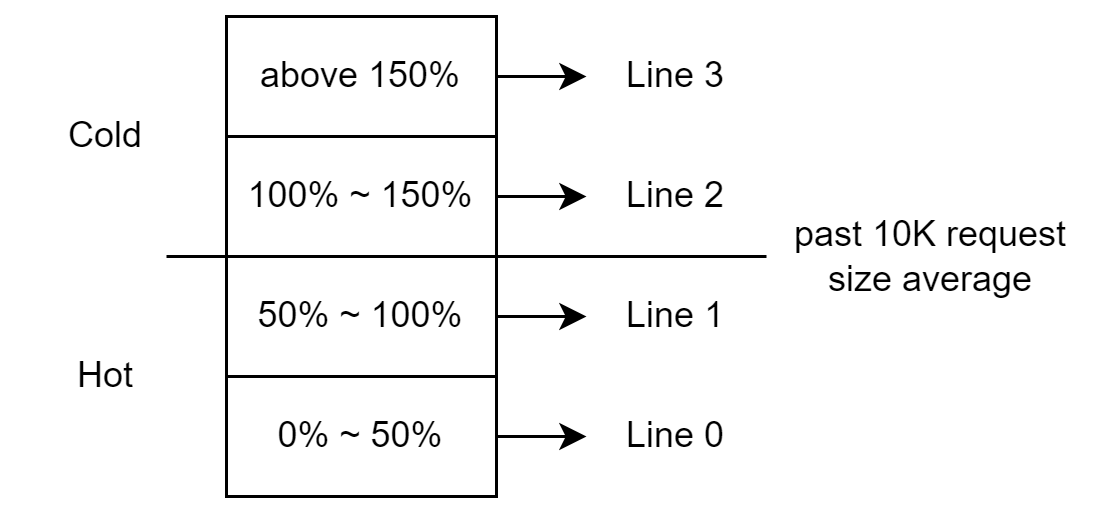
\includegraphics[width=0.7\textwidth]{picture/ch3/hot_cold.png}
    \caption{熱門資料與冷門資料}
    \label{f3.2}
\end{figure}

\subsection{擷取 Request 大小並判斷分群}\label{s3.2.2}
\indent
在得到 Request 大小時,我們需要從檔案系統傳給 LightNVM 的資料結構 bio 之中,找到 Request 大小的值;之後再以 Request 大小與平均值,判斷當下的 Request 屬於哪一類。
\begin{figure}[H]
    \centering
    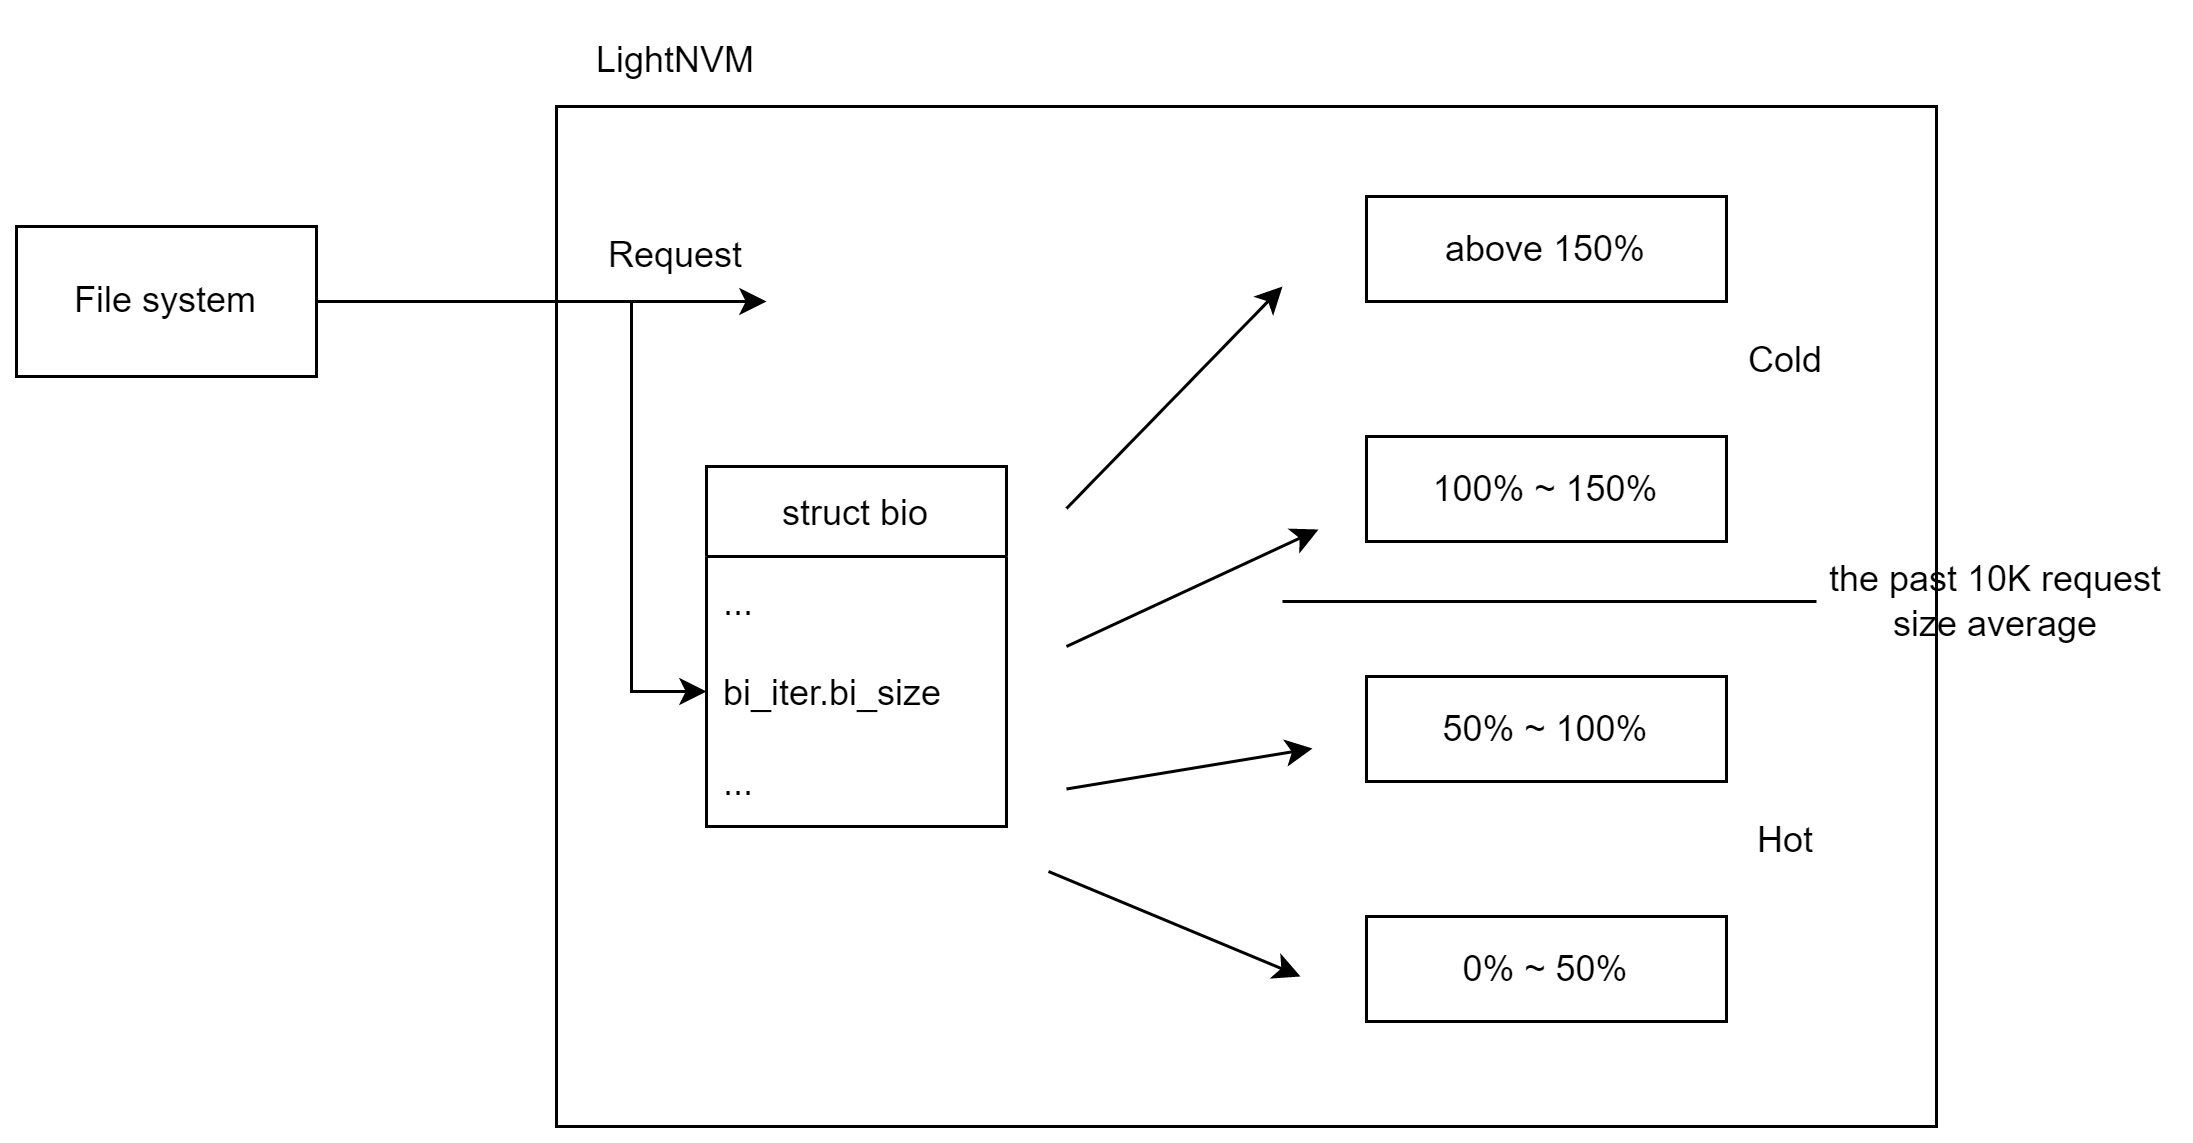
\includegraphics[width=1\textwidth]{picture/ch3/get_rq_size_hot_cold.png}
    \caption{判斷 Request 分群}
    \label{f3.3}
\end{figure}


\subsection{計算平均值}\label{s3.2.3}
\indent
在判斷完分群之後,我們需要拿剛剛得到的 Request 大小與平均值計算出新的平均值;由於我們需要前一萬筆 Request 大小的平均值,所以得到大小之後將其乘以 0.0001 倍再與我們加入 LightNVM 的平均值乘以 0.9999 倍之後相加,之後下一次檔案系統傳送 Request 進來時,就可以繼續用來判斷分群。
\begin{figure}[H]
    \centering
    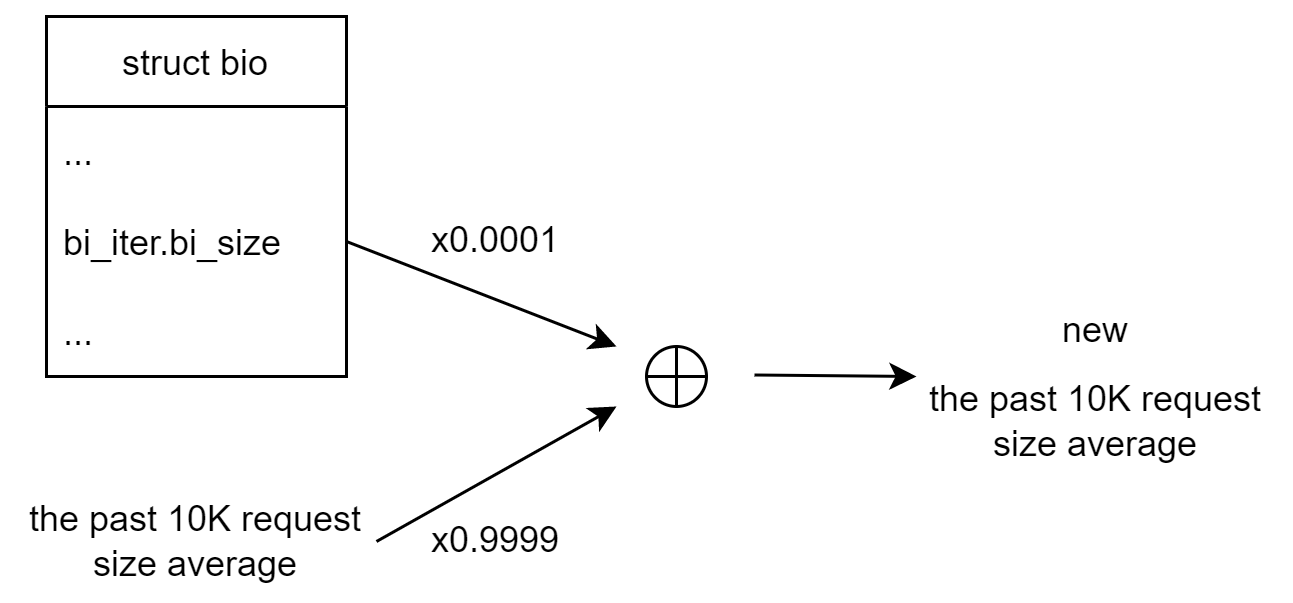
\includegraphics[width=0.8\textwidth]{picture/ch3/new_average.png}
    \caption{計算新平均值}
    \label{f3.4}
\end{figure}

\subsection{將 Request 所屬分群的資訊放入 Ring Buffer 中}\label{s3.2.4}
\indent
LightNVM 在接到檔案系統的 Request 之後,會將 Request 的資料拆解成數個 Page,每個 Page 都會記錄成 Ring Buffer 一個 Entry 之中,之後便會喚醒 LightNVM 背景的 write thread,從 Ring Buffer 存取剛剛放進去的 Entry,來得知寫入的資料位於 Host 記憶體,我們在這個 Entry 之中加入要存入哪個 Line,也就是冷熱分群的資訊,以便之後的 write thread 使用。

\begin{figure}[H]
    \centering
    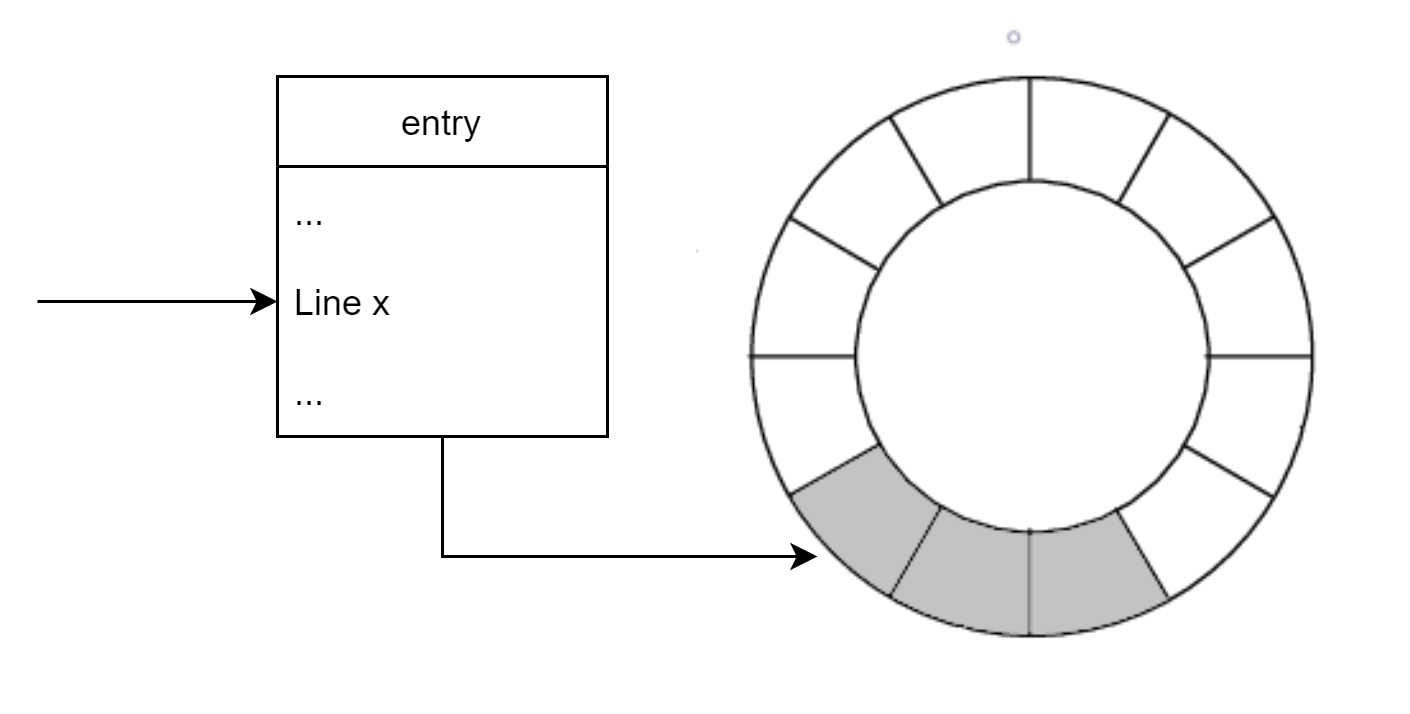
\includegraphics[width=0.7\textwidth]{picture/ch3/store_line_in_ring_buffer_entry.png}
    \caption{將分群資訊放入 Ring Buffer 的單位資料結構(Entry)}
    \label{f3.5}
\end{figure}

\section{實際寫入之過程}\label{s3.3}
\indent
LightNVM 的 Write Thread 被喚醒之後,會從剛剛紀錄到 Ring Buffer 之中的 Entry 得知要寫入的資料在哪裡,而我們也跟著得知剛剛我們放入的資訊,也就是每個 Entry 所屬的冷熱分群,接著我們將所有當次所提取的 Entry 的所屬冷熱分群總和之後取平均,得到的平均值就是我們最後寫入的 Line,最後我們將 Line 切換到我們的目標之後,LightNVM 就會根據我們所提供的 Line 來做 allocation,最終傳給 Open Channel SSD。

\subsection{從 Ring Buffer 中蒐集 Entry}\label{s3.3.1}
\indent
每次 LightNVM 從 Ring Buffer 之中抽取出的 Entry 數量不一定一樣,假設這次會取四個 Entry 的資料,分別所屬為 Line 3、2、1、2,那最後平均值是 2。

\begin{figure}[H]
    \centering
    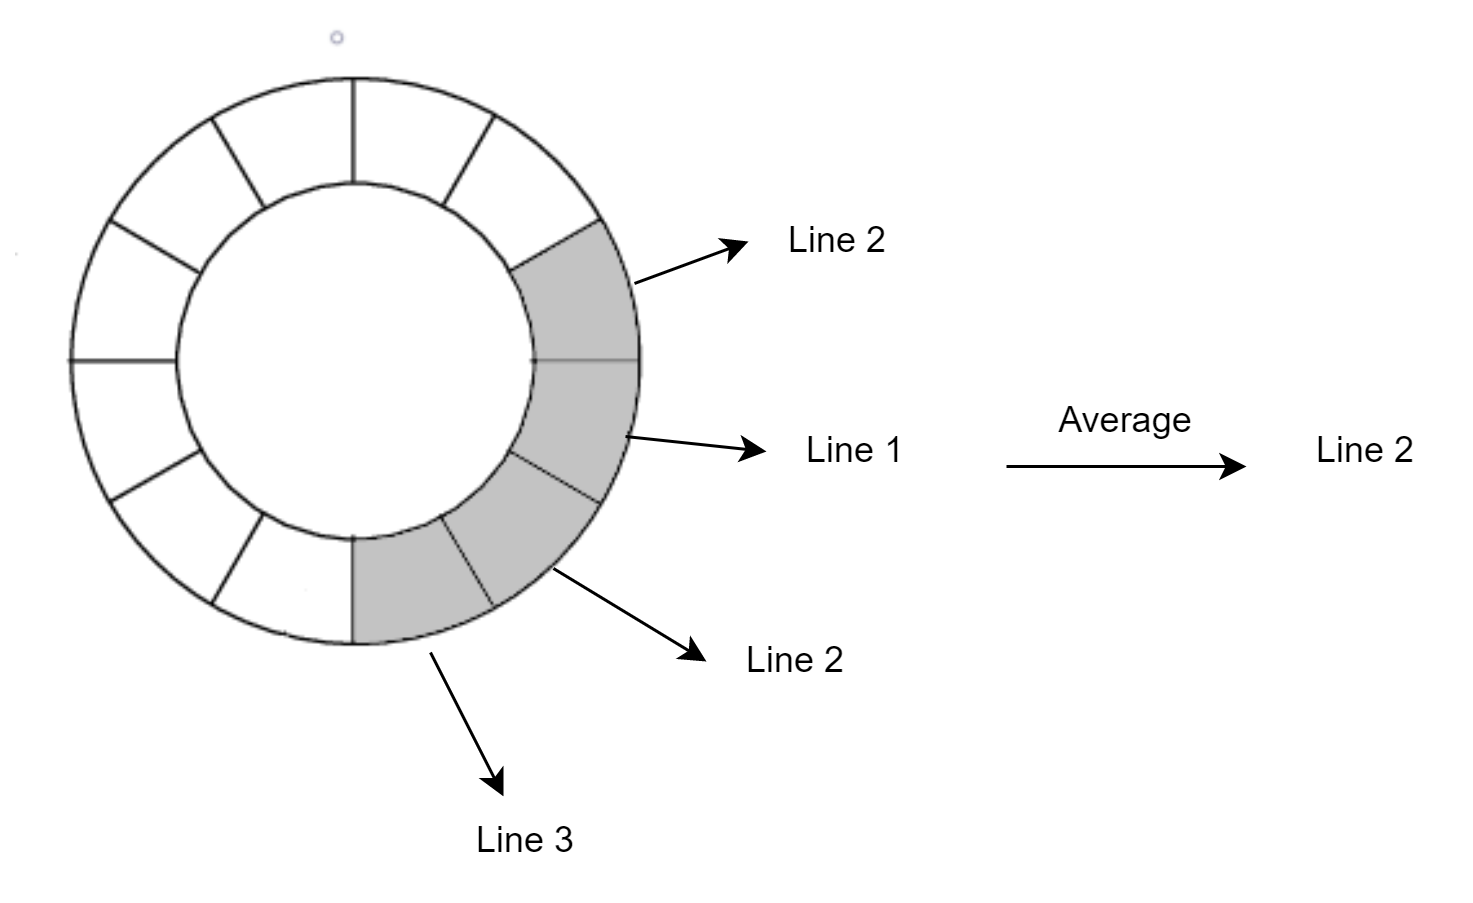
\includegraphics[width=0.7\textwidth]{picture/ch3/get_entry_from_ring_buffer.png}
    \caption{從數個 Entry 取出 Line 之後平均}
    \label{f3.6}
\end{figure}

\subsection{切換 Line 之後傳送給 Open Channel SSD}\label{s3.3.2}
\indent
按照剛剛計算的平均值切換 Line 之後,LightNVM 會根據我們指定的 Line 做 Allocation,最後將資料以及位置往下傳給 Open Channel SSD(圖例延續 \ref{s3.3.1})。
\begin{figure}[H]
    \centering
    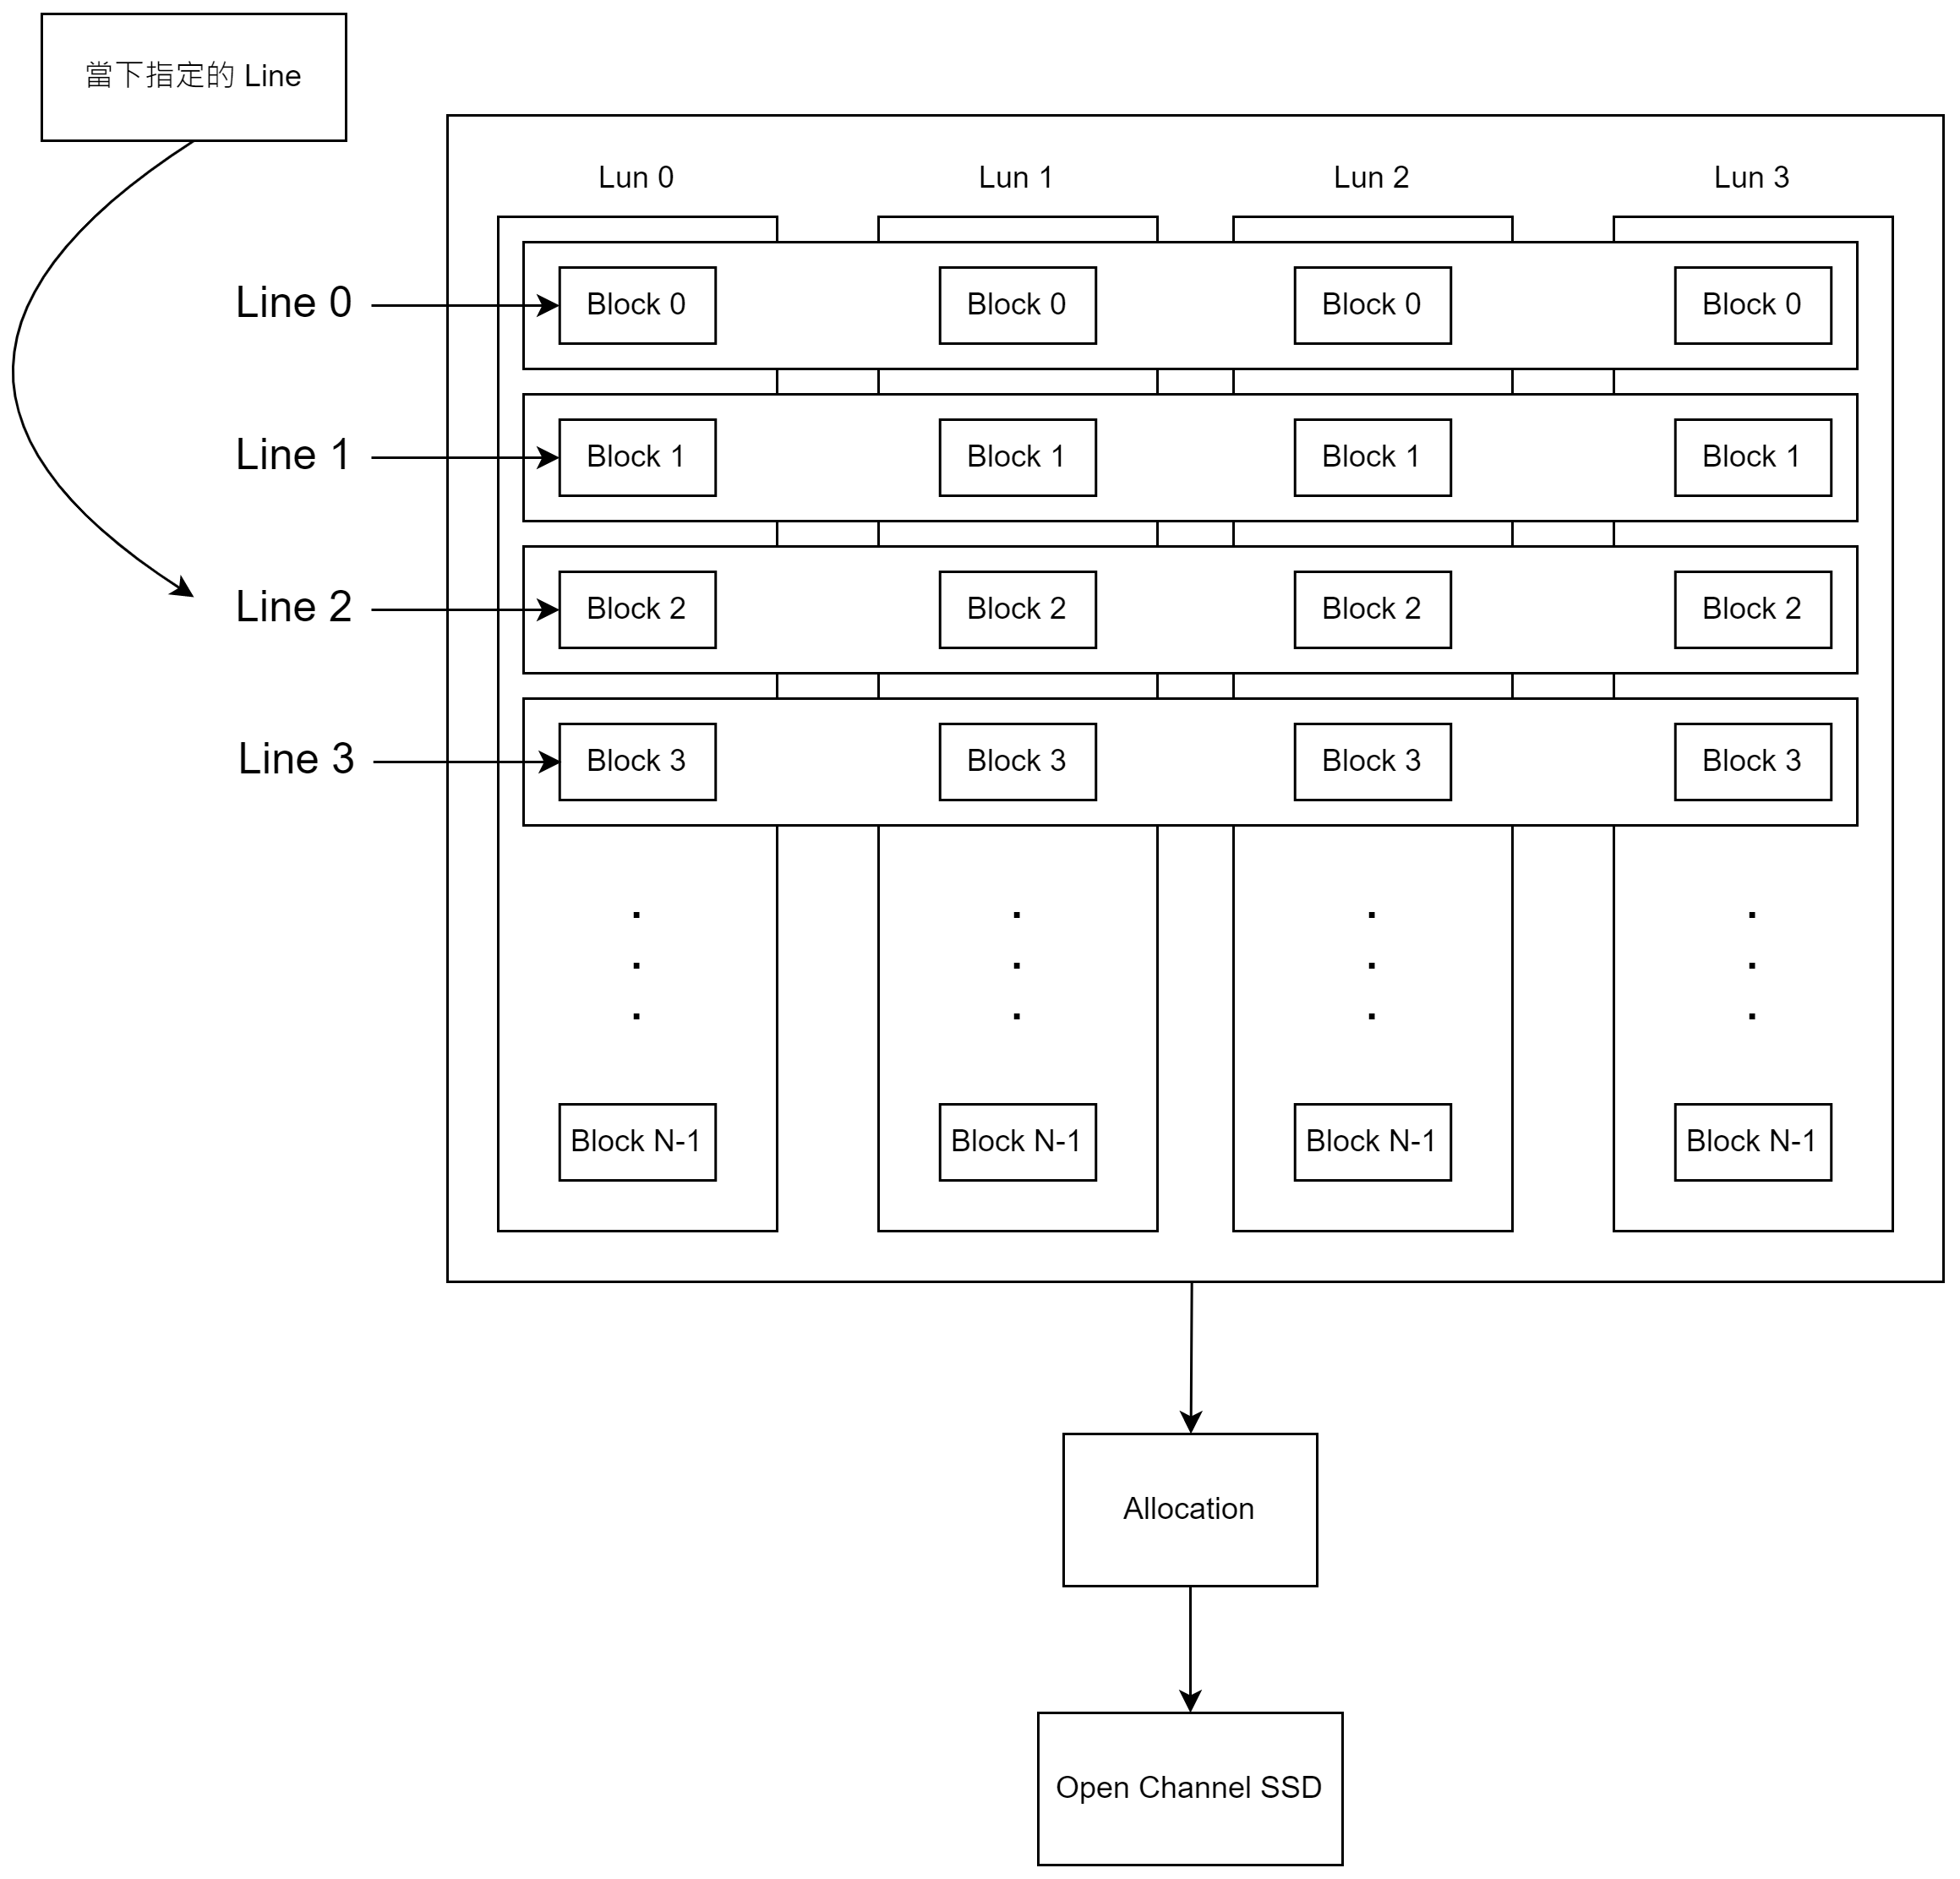
\includegraphics[width=1\textwidth]{picture/ch3/switch_line_to_opssd.drawio.png}
    \caption{切換 Line 之後 Allocation,最後傳給 Open Channel SSD}
    \label{f3.7}
\end{figure}
%\subsection{建立開發外掛程式之環境}
%\indent
%Plug-in Development Environment(PDE)\cite{PDE}是Eclipse中提供開發人員進行外掛程式開發的工具,其中提供了多種協助開發的功能,例如:創立專案、除錯、測試、建置專案、部屬等等。本論文將在PDE中引入既有外掛程式之專案,進行新重構功能之擴充。

%\subsection{利用Eclipse中延伸點與應用程式介面進行擴充}
%\indent
%\ref{s2.4}節中提及了Eclipse的擴充機制,而Eclipse中含有十分豐富的延伸點與各種應用程式介面,透過不同的延伸點與應用程式介面的結合,外掛程式可以更多元地使用Eclipse上的各種功能,例如:監聽使用者操作進而做出後續反應、取得工作區檔案中的各項資訊提供外掛程式使用等等。本論文透過此擴充機制能夠更加簡化使用者重構之動作,且更方便地新增重構功能。

%\subsection{增加command元素}\label{s3.4.3}
%\indent
%在Eclipse中command是一個行為的描述,但與實際行為操作並無相關,其行為操作是由handler所定義,而一個command可以擁有多個handler,但在一個時間點上只會將行為託付給一個handler。Eclipse提供了commands的延伸點,開發人員能夠藉此新增command以及定義其種類。本論文將為已有三個command的commands延伸點進行擴充,新增兩個command,分別為抽取重複步驟成為新關鍵字、移動關鍵字宣告,後續將新增handler為其定義實際行為。圖\ref{f3.9}為現有commands之延伸點。
%
%\begin{figure}[H]
%    \centering
%    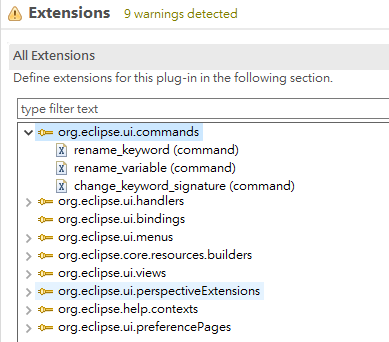
\includegraphics[width=0.8\textwidth]{picture/command_extension.PNG}
%    \caption{外掛程式現有之commands延伸點3}
%    \label{f3.9}
%\end{figure}
%
%\subsection{透過handler定義新command的行為}
%\indent
%Eclipse提供了handlers的延伸點,讓開發人員能夠進行handler與command的連接,並且設定handler在不同條件下為啟用、禁用或非活動的狀態,如果handler處於禁用狀態,儘管收到了command的委託,也不會執行,而處於非活動的狀態時,command將不會被委託至此handler,因此在啟用狀態下,command將會委託此handler執行行為。本論文將為已有三個handler的handlers延伸點新增兩個handler,並將其與\ref{s3.4.3}節中的command進行連接,完成相對應的重構行為。圖\ref{f3.10}為現有handlers之延伸點。
%
%\begin{figure}[H]
%    \centering
%    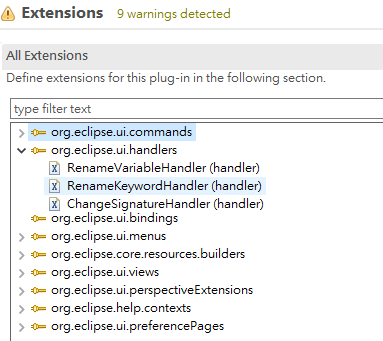
\includegraphics[width=0.8\textwidth]{picture/handler_extension.PNG}
%    \caption{外掛程式現有之handlers延伸點}
%    \label{f3.10}
%\end{figure}
%
%\subsection{將新command與選單介面結合}
%\indent
%Eclipse提供了menus的延伸點,讓開發人員能夠將客製化的選單新增至Eclipse框架上,提供使用者能夠操作其所需之功能,其中提供了以下幾種選單種類:
%
%\begin{itemize}
%
%\item\textbf{主選單(Main menu)}
%
%\item\textbf{主工具列(Main toolbars)}
%
%\item\textbf{修剪選單(Trim)}
%
%\item\textbf{視圖選單/工具列(View menus/Toolbars)}
%
%\end{itemize}
%
%\indent
%此外選單介面可與不同元件結合,例如:control、command、menu等等,讓客製化選單能夠更加多元。本論文將於現有menus延伸點的客製化選單中,結合\ref{s3.4.3}節中所新增之command,讓使用者能夠依照其需求選擇選單中的功能,並將command委託至handler執行。圖\ref{f3.11}為現有menus之延伸點。
%
%\begin{figure}[H]
%    \centering
%    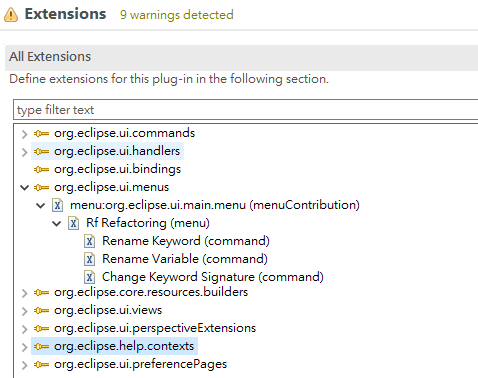
\includegraphics[width=0.8\textwidth]{picture/menu_extension.PNG}
%    \caption{外掛程式現有之menus延伸點}
%    \label{f3.11}
%\end{figure}

%\subsection{透過視圖及視窗協助重構功能執行}
%\indent
%Eclipse提供了views延伸點,開發人員可藉此新增客製化的視圖(View),而視圖為工作區內的可視化元件,其可被用來顯示command執行結果資訊或新增額外的使用者元件等等,圖\ref{f3.12}為現有外掛程式的客製化視圖,其提供使用者選擇所要重新命名的參考。本論文將於現有views延伸點新增兩個不同的客製化視圖,分別提供使用者選擇重複步驟或目標檔案,以此協助重構功能之執行。
%
%\begin{figure}[H]
%    \centering
%    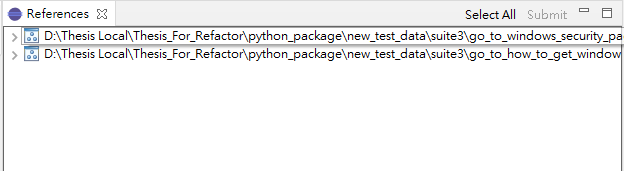
\includegraphics[width=1.0\textwidth]{picture/choose_keyword_view.PNG}
%    \caption{現有外掛程式的客製化視圖}
%    \label{f3.12}
%\end{figure}
%
%\indent
%視窗(Dialog)是SWT(Standard Widget Toolkit)\cite{SWT}中所提供的視窗元件,其可透過開發人員自行設計介面,以達到所需之功能,圖\ref{f3.13}為現有外掛程式的客製化視窗,其提供使用者輸入重新命名的關鍵字名稱。本論文將新增兩個視窗介面,提供使用者創建新關鍵字及用新關鍵字取代重複步驟之功能使用,協助整體重構功能之執行。
%
%\begin{figure}[H]
%    \centering
%    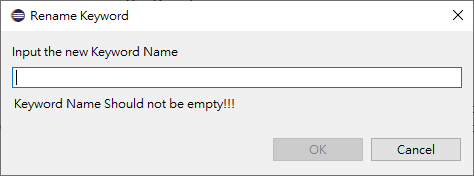
\includegraphics[width=0.7\textwidth]{picture/Rename_keyword_dialog.PNG}
%    \caption{現有外掛程式的客製化視窗}
%    \label{f3.13}
%\end{figure}
\chapter{案例分析}
\section{案例實驗設計}
\indent
本論文將以自行設計之Microsoft網頁相關測試專案作為實驗腳本,其中含有十一個測試套件、七個測試資源,是屬於規模較小的測試專案,此實驗將以團隊最常使用的Visual Studio Code搜尋取代工具及擴充後之RF Refactoring進行重構,其重構方法為抽取測試腳本之重複步驟成為新關鍵字及移動關鍵字宣告兩種。

\indent
本論文將參考陳昱仁論文\cite{Experiment_Settings}實驗分析中的實驗設計方法,邀請國立台北科技大學軟體系統實驗室之測試團隊成員,協助使用兩種工具進行重構並比較其時間差異,以此確認擴充後之重構工具對於團隊是否有實質之幫助。在開始測驗之前,將會帶領每位測試人員了解該測試專案所要測試的網頁內容,使其對測試專案先有一定的了解。因為現有環境上的限制,只能請測試人員務必於只有一人的環境中進行測驗,並且確保其餘可能影響實驗準確性之外在因素皆不存在,例如:手機、通訊軟體等等,最後為每位測試人員解釋各個案例狀況後即開始進行測驗。

\section{案例一:抽取測試腳本中的重複步驟成為新關鍵字並引入所需測試資源}\label{s5.1}
\indent
程式碼\ref{l5.1}為測試專案的測試套件之一,其含有一個測試案例,用來測試前往Windows安全性頁面之功能,並且測試其功能正常後,於報表中印出歡迎相關之訊息。程式碼\ref{l5.2}同為測試專案中的測試套件,同樣含有一個測試案例,用來測試前往Windows10功能頁面之功能,於功能驗證完成後,在報表中印出歡迎相關之訊息。

\indent
比對程式碼\ref{l5.1}(18-20行)及程式碼\ref{l5.2}(18-20行)可以發現,其在於功能驗證後都會印出歡迎相關之訊息,因此可以將它們認定為重複步驟並進行重構。此測試專案中共有四個測試案例都擁有重複之步驟,需要將其抽取成新關鍵字並取代後,引入其所需之測試資源,因此本論文邀請五位測試團隊成員依照下列小節之方式,進行相對應之重構,並於後續比較其使用差異。

\begin{lstlisting}[caption=前往Windows安全性頁面之測試套件, label={l5.1}]
9   *** Variables ***
10  @{welcomeTaipei} =    Welcome    To    Taipei
11  
12  *** Test Cases ***
13  Go To "Windows Security" Page And Log Welcome Text
14      Go To Windows Page
15      Open Windows 10 Menu
16      Go To "Windows Security" Page
17      "Windows Security" Page Should Be Visible
18      FOR    ${var}    IN    @{welcomeTaipei}
19          Log Double Text    ${var}
20      END
21      [Teardown]    Close Browser
\end{lstlisting}

\begin{lstlisting}[caption=前往Windows10功能頁面之測試套件, label={l5.2}]
9   *** Variables ***
10  @{welcomeTainan} =    Welcome    To    Tainan
11
12  *** Test Cases ***
13  Go To "Windows 10 features" Page And Log Welcome Text
14      Go To Windows Page
15      Open Windows 10 Menu
16      Go To "Windows 10 features" Page
17      "Windows 10 features" Page Should Be Visible
18      FOR    ${var}    IN    @{welcomeTainan}
19          Log Double Text    ${var}
20      END
21      [Teardown]    Close Browser
\end{lstlisting}
\newpage

\subsection{使用Visual Studio Code搜尋取代工具}\label{s5.1.1}
\indent
首先利用Visual Studio Code(VSCode)將重複步驟複製至目標測試資源中,以其做了什麼為新關鍵字之名稱,且將未宣告於步驟內之變數作為新關鍵字之參數,藉此創立新關鍵字,結果如程式碼\ref{l5.3}。後續於搜尋工具中,以重複步驟之關鍵字為搜尋目標,搜尋結果如圖\ref{f5.1}所示,其中一個搜尋結果為關鍵字之宣告,非所需之重複步驟故不取代,其餘四個結果分別與重複步驟之參數數量、關鍵字順序及關鍵字名稱相同,因此以新關鍵字進行取代。

\indent
後續於已進行重複步驟取代之測試套件,檢查其是否有引入新關鍵字所需之測試資源,為未引入者進行引入之動作。

\begin{lstlisting}[caption=新關鍵字架構, label={l5.3}]
Log Welcome Text
    [Arguments]    ${welcomeTexts}
    FOR    ${var}    IN    @{welcomeTexts}
        Log Double Text    ${var}
    END
\end{lstlisting}

\begin{figure}[H]
   \centering
   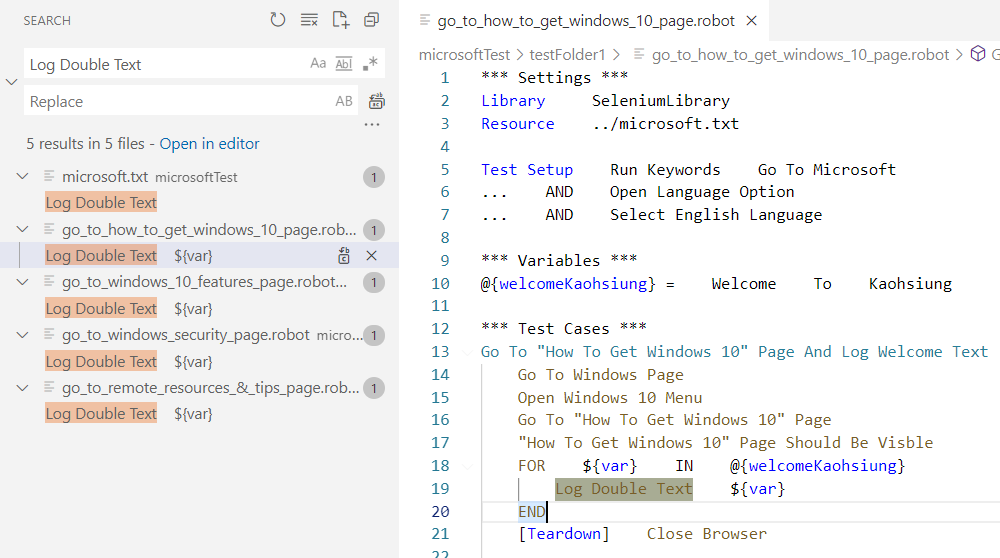
\includegraphics[width=0.9\textwidth]{picture/ch5/vscode_search_in_case1.PNG}
   \caption{重複步驟搜尋結果}
   \label{f5.1}
\end{figure}

%\begin{figure}[H]
%	\centering
%	\begin{minipage}[b]{0.43\textwidth}
%		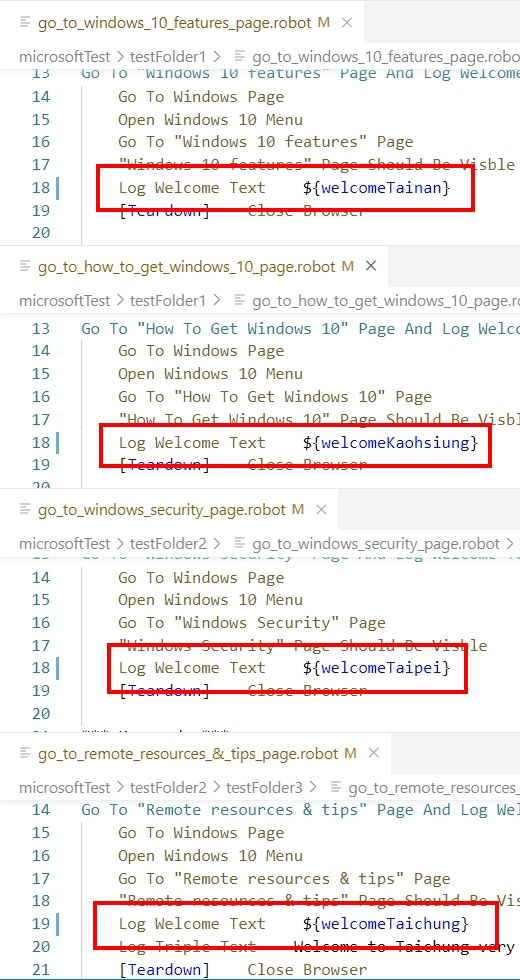
\includegraphics[width=1.05\textwidth]{picture/ch5/After_replace_with_new_keyword_in_case1.png}
%		\caption{關鍵字取代重複步驟後結果}
%		\label{f5.2}
%	\end{minipage}
%	\begin{minipage}[b]{0.53\textwidth}
%		\centering
%		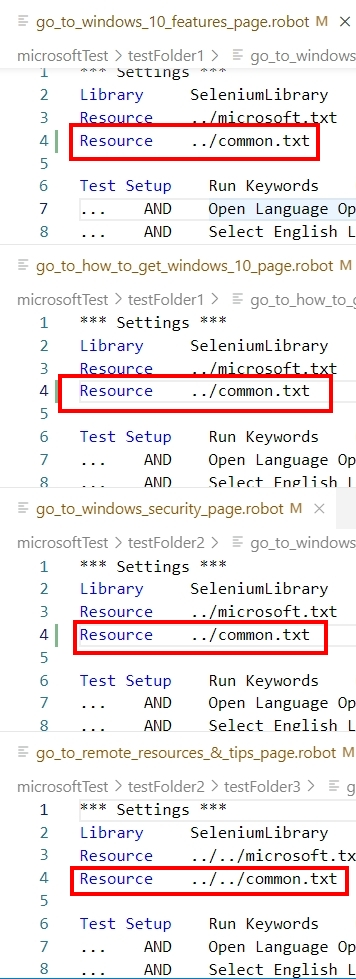
\includegraphics[width=0.85\textwidth]{picture/ch5/Import_resource_in_case1.png}
%		\caption{引入新關鍵字所需之測試資源結果}
%		\label{f5.3}
%	\end{minipage}
%\end{figure}

\subsection{使用擴充後之RF Refactoring}\label{s5.1.2}
\indent
後續使用擴充後之RF Refactoring的Wrap Steps As A New Keyword功能重構\ref{s5.1}節所提及之重複步驟,選取其中一個測試套件中的重複步驟,其將會自動把未宣告於步驟中的變數加入新關鍵字的參數,如圖\ref{f5.4}所示,於此視窗可以同時決定新關鍵字之名稱,並且創立新關鍵字於圖\ref{f5.5}視圖中所選擇之檔案。根據專案下所檢查出含有重複步驟的測試套件,其可在圖\ref{f5.6}之視圖中選擇要以新關鍵字取代之重複步驟,並且為每個要使用的新關鍵字決定其參數實際值,以此完成重複步驟之取代,最後RF Refactoring將自動引入新關鍵字所需之測試資源。

\begin{figure}[H]
    \centering
    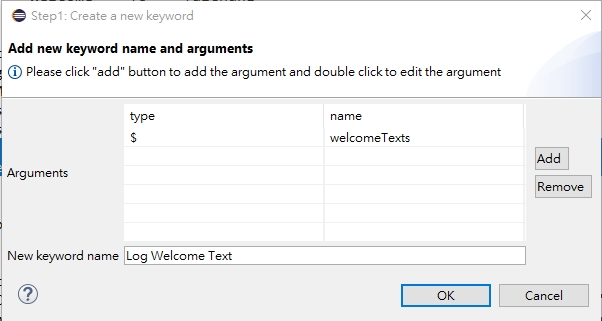
\includegraphics[width=0.7\textwidth]{picture/ch5/Eclipse_create_keyword_in_case1.png}
    \caption{創立新關鍵字視窗結果}
    \label{f5.4}
\end{figure}

\begin{figure}[H]
    \centering
    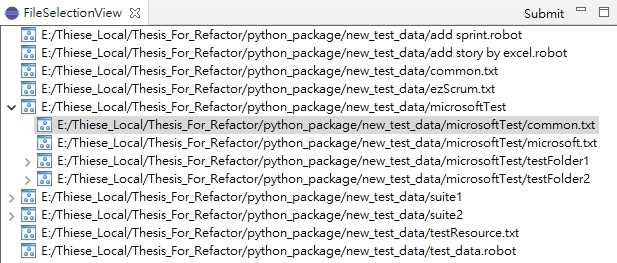
\includegraphics[width=0.7\textwidth]{picture/ch5/Eclipse_choose_file_to_create_keyword_in_case1.png}
    \caption{專案下檔案顯示視圖結果}
    \label{f5.5}
\end{figure}

\begin{figure}[H]
    \centering
    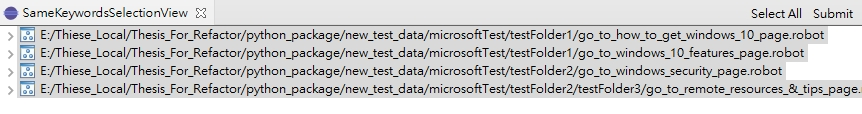
\includegraphics[width=0.7\textwidth]{picture/ch5/Eclipse_choose_duplicate_steps_in_case1.png}
    \caption{搜尋重複步驟結果之視圖}
    \label{f5.6}
\end{figure}

%\begin{figure}[H]
%	\centering
%	\begin{minipage}[b]{0.43\textwidth}
%		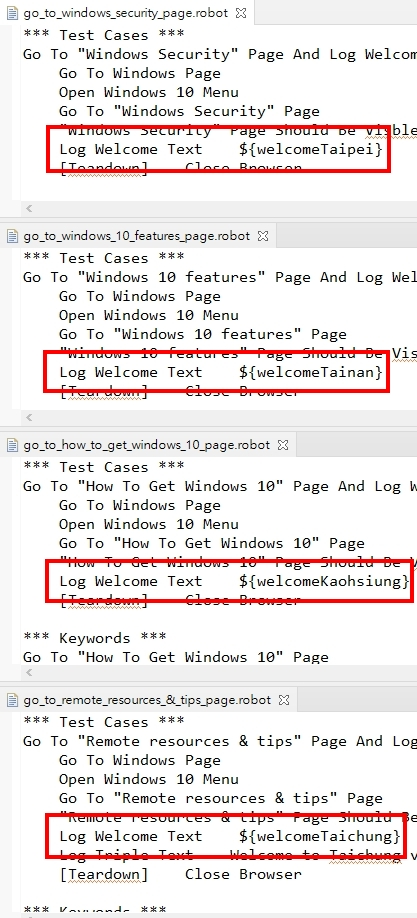
\includegraphics[width=1.05\textwidth]{picture/ch5/Eclipse_replace_result_in_case1.png}
%		\caption{關鍵字取代重複步驟後結果}
%		\label{f5.7}
%	\end{minipage}
%	\begin{minipage}[b]{0.53\textwidth}
%		\centering
%		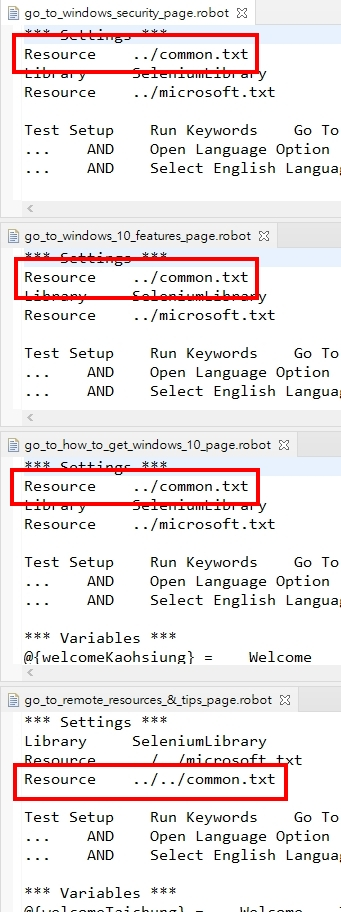
\includegraphics[width=0.85\textwidth]{picture/ch5/Eclipse_Import_resource_result_in_case1.png}
%		\caption{引入新關鍵字所需之測試資源結果}
%		\label{f5.8}
%	\end{minipage}
%\end{figure}

\subsection{重構工具使用之比較}

\begin{table}[H]
    \begin{center}
    \caption{使用兩種工具包裹重複步驟成為新關鍵字並引入所需測試資源之比較}\label{t5.1}
        \begin{tabular}{|c|c|c|}\hline
                             & 使用VSCode重構花費之時間    & 使用擴充後之RF Refactoring重構花費之時間    \\\hline
        測試人員1           & 06m02s          & 03m24s    \\\hline
        測試人員2           & 05m12s          & 04m20s    \\\hline
        測試人員3           & 07m31s          & 04m20s    \\\hline
        測試人員4           & 06m20s          & 04m59s    \\\hline
        測試人員5           & 06m29s          & 06m07s    \\\hline
\textbf{平均時間}           & \textbf{06m18s} & \textbf{04m38s}    \\\hline
        \end{tabular}
    \end{center}
\end{table}
\indent
表\ref{t5.1}為紀錄團隊測試人員使用兩種不同工具進行此重構之比較,從表中可見每一位測試人員根據經驗之不同,使用VSCode進行重構所花費之時間也略微不同,平均大約花費了6分18秒,並且重構過程中,測試人員有三位不小心忽視了新關鍵字所需之測試資源,導致測試失敗;而使用擴充後之RF Refactoring重構時,平均大約花費了4分38秒,並且未有測試資源沒被引入之狀況發生。由此比較可發現,使用擴充後之RF Refactoring進行此重構時,因為不需要手動搜尋重複步驟以及檢查所需之測試資源是否引入,能夠花費較少的時間,其大約減少了26.4\%的時間,並且較不容易發生錯誤。

\section{案例二:移動測試資源中的關鍵字宣告並引入所需測試資源}\label{s5.2}
\indent
程式碼\ref{l5.4}為測試專案的測試套件之一,其中第5行之Go To Microsoft關鍵字於其他測試套件剛好也需要使用,因此必須將其之宣告移動至共用之測試資源,以便其他測試套件使用。在移動到目標測試資源後,必須檢查原先已使用此關鍵字之四個測試套件是否都有引入其所需之測試資源,避免發生未宣告關鍵字之錯誤。

\indent
根據此案例之重構,本論文邀請與\ref{s5.1}節相同之五位測試團隊成員使用下列小節之方式,進行相對應之重構,最後比較其使用差異。

\begin{lstlisting}[caption=前往如何取得Windows10頁面之測試套件, label={l5.4}]
1   *** Settings ***
2   Library     SeleniumLibrary
3   Resource    ../microsoft.txt
4
5   Test Setup    Run Keywords    Go To Microsoft
6   ...    AND    Open Language Option
7   ...    AND    Select English Language

8   *** Variables ***
9   @{welcomeKaohsiung} =    Welcome    To    Kaohsiung
10
11  *** Test Cases ***
12  Go To "How To Get Windows 10" Page And Log Welcome Text
13      Go To Windows Page
14      Open Windows 10 Menu
15      Go To "How To Get Windows 10" Page
16      "How To Get Windows 10" Page Should Be Visible
17      Log Welcome Text    ${welcomeKaohsiung}
18      [Teardown]    Close Browser
\end{lstlisting}

\subsection{使用Visual Studio Code搜尋取代工具}
\indent
首先利用VSCode將需要移動之關鍵字宣告於其所在檔案中移除,並在共用測試資源上完整複製遭移除之關鍵字宣告,後續於搜尋工具之視窗,以被移動之關鍵字名稱進行搜尋,搜尋結果如圖\ref{f5.9}所示,其中一個搜尋結果為關鍵字之宣告的,故不需檢查,其餘結果皆為原先已使用此關鍵字之測試套件。接著於每個測試套件中搜尋是否有引入共用之測試資源,如否則為其引入以避免測試錯誤。

\begin{figure}[H]
    \centering
    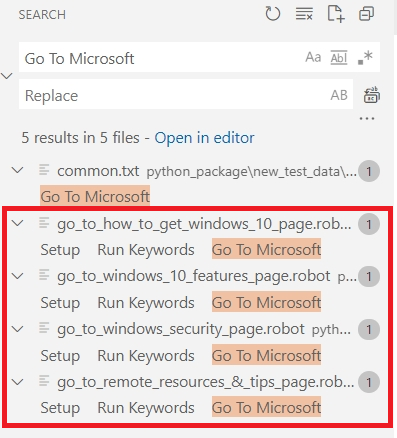
\includegraphics[width=0.35\textwidth]{picture/ch5/Search_using_keyword_in_case2.png}
    \caption{搜尋使用被移動關鍵字之測試套件結果}
    \label{f5.9}
\end{figure}

%\begin{figure}[H]
%	\centering
%	\begin{minipage}[b]{0.5\textwidth}
%		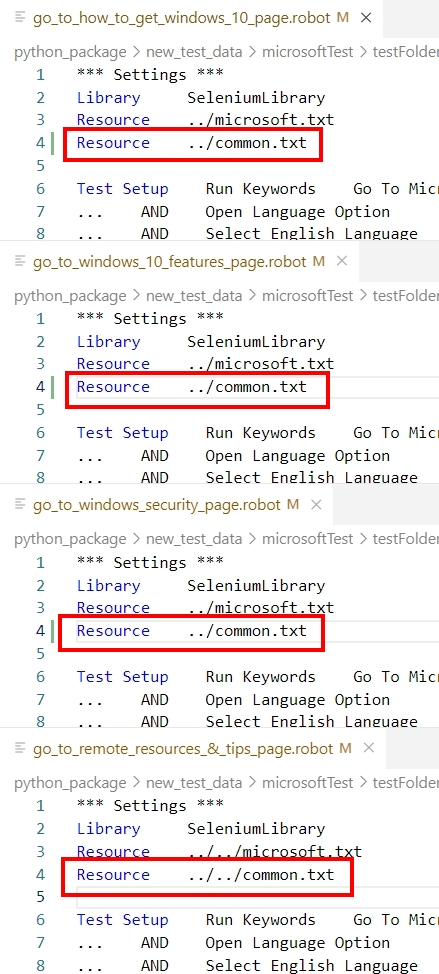
\includegraphics[width=0.8\textwidth]{picture/ch5/Import_resource_in_case2.png}
%		\caption{引入關鍵字所需之測試資源結果}
%		\label{f5.10}
%	\end{minipage}
%	\begin{minipage}[b]{0.48\textwidth}
%		\centering
%		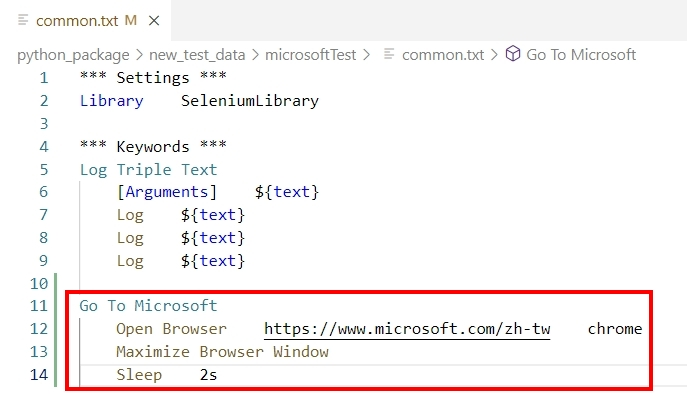
\includegraphics[width=1.2\textwidth]{picture/ch5/Move_keyword_result_in_case2.png}
%		\caption{關鍵字宣告移動之結果}
%		\label{f5.11}
%	\end{minipage}
%\end{figure}

\subsection{使用擴充後之RF Refactoring}
\indent
接著使用擴充後之RF Refactoring的Move Keyword Defined To Another File功能重構\ref{s5.2}節所提及的需移動之關鍵字宣告,選取其關鍵字名稱後,即可將關鍵字宣告移動至圖\ref{f5.12}視圖中所選取之目標檔案,後續RF Refactoring將自動為原先已使用此關鍵字之測試套件引入所需測試資源。

\begin{figure}[H]
    \centering
    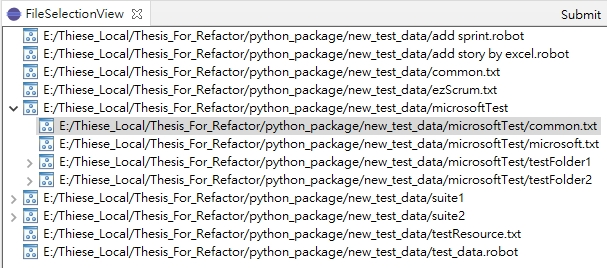
\includegraphics[width=0.7\textwidth]{picture/ch5/Eclipse_choose_file_in_case2.png}
    \caption{專案下全部測試檔案之視圖}
    \label{f5.12}
\end{figure}

%\begin{figure}[H]
%	\centering
%	\begin{minipage}[b]{0.48\textwidth}
%		\centering
%		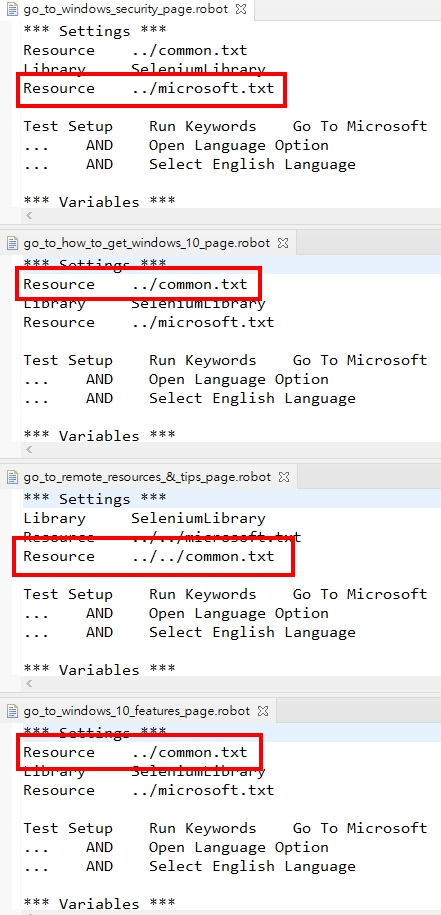
\includegraphics[width=0.9\textwidth]{picture/ch5/Eclipse_import_resource_in_case2.png}
%		\caption{引入關鍵字所需測試資源之結果}
%		\label{f5.13}
%	\end{minipage}
%	\begin{minipage}[b]{0.5\textwidth}
%		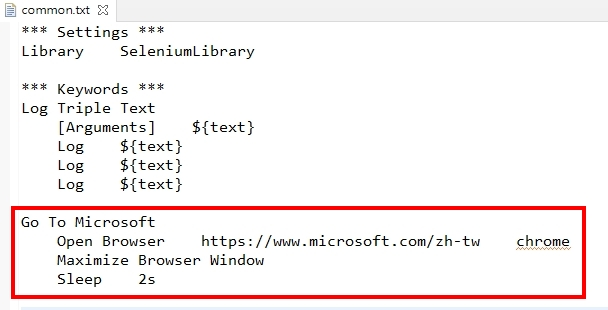
\includegraphics[width=1.2\textwidth]{picture/ch5/Eclipse_move_keyword_result_in_case2.png}
%		\caption{關鍵字宣告移動之結果}
%		\label{f5.14}
%	\end{minipage}
%\end{figure}

\subsection{重構工具使用之比較}

\begin{table}[H]
    \begin{center}
    \caption{使用兩種工具移動關鍵字宣告並引入所需測試資源之比較}\label{t5.2}
        \begin{tabular}{|c|c|c|}\hline
                & 使用VSCode重構花費之時間 & 使用擴充後之RF Refactoring重構花費之時間    \\\hline
        測試人員1      & 01m14s             & 00m26s    \\\hline
        測試人員2      & 01m35s             & 00m18s    \\\hline
        測試人員3      & 01m17s             & 00m22s    \\\hline
        測試人員4      & 01m00s             & 00m26s    \\\hline
        測試人員5      & 02m02s             & 00m41s    \\\hline
\textbf{平均時間}      & \textbf{01m25s}    & \textbf{00m26s}    \\\hline
        \end{tabular}
    \end{center}
\end{table}
\indent
表\ref{t5.2}為紀錄團隊測試人員使用兩種不同工具進行此重構之比較,從表中可發現,使用VSCode進行重構時,平均花費了1分25秒,且有兩位測試人員對於部分測試套件有錯誤引入關鍵字所需測試資源之相對路徑,導致測試錯誤;而使用擴充後之RF Refactoring重構時,平均花費了26秒,且引入所需測試資源之路徑皆為正確。從此比較可發現,使用擴充後之RF Refactoring進行此重構時,因為不需要自我檢查測試套件是否都有引入所需之測試資源,能夠花費較少的時間,其大約減少了69.4\%的時間,並且較不容易因人為檢查缺漏而發生錯誤。
\chapter{案例分析}
\section{案例實驗設計}
\indent
本論文將以自行設計之Microsoft網頁相關測試專案作為實驗腳本,其中含有十一個測試套件、七個測試資源,是屬於規模較小的測試專案,此實驗將以團隊最常使用的Visual Studio Code搜尋取代工具及擴充後之RF Refactoring進行重構,其重構方法為抽取測試腳本之重複步驟成為新關鍵字及移動關鍵字宣告兩種。

\indent
本論文將參考陳昱仁論文\cite{Experiment_Settings}實驗分析中的實驗設計方法,邀請國立台北科技大學軟體系統實驗室之測試團隊成員,協助使用兩種工具進行重構並比較其時間差異,以此確認擴充後之重構工具對於團隊是否有實質之幫助。在開始測驗之前,將會帶領每位測試人員了解該測試專案所要測試的網頁內容,使其對測試專案先有一定的了解。因為現有環境上的限制,只能請測試人員務必於只有一人的環境中進行測驗,並且確保其餘可能影響實驗準確性之外在因素皆不存在,例如:手機、通訊軟體等等,最後為每位測試人員解釋各個案例狀況後即開始進行測驗。

\section{案例一:抽取測試腳本中的重複步驟成為新關鍵字並引入所需測試資源}\label{s5.1}
\indent
程式碼\ref{l5.1}為測試專案的測試套件之一,其含有一個測試案例,用來測試前往Windows安全性頁面之功能,並且測試其功能正常後,於報表中印出歡迎相關之訊息。程式碼\ref{l5.2}同為測試專案中的測試套件,同樣含有一個測試案例,用來測試前往Windows10功能頁面之功能,於功能驗證完成後,在報表中印出歡迎相關之訊息。

\indent
比對程式碼\ref{l5.1}(18-20行)及程式碼\ref{l5.2}(18-20行)可以發現,其在於功能驗證後都會印出歡迎相關之訊息,因此可以將它們認定為重複步驟並進行重構。此測試專案中共有四個測試案例都擁有重複之步驟,需要將其抽取成新關鍵字並取代後,引入其所需之測試資源,因此本論文邀請五位測試團隊成員依照下列小節之方式,進行相對應之重構,並於後續比較其使用差異。

\begin{lstlisting}[caption=前往Windows安全性頁面之測試套件, label={l5.1}]
9   *** Variables ***
10  @{welcomeTaipei} =    Welcome    To    Taipei
11  
12  *** Test Cases ***
13  Go To "Windows Security" Page And Log Welcome Text
14      Go To Windows Page
15      Open Windows 10 Menu
16      Go To "Windows Security" Page
17      "Windows Security" Page Should Be Visible
18      FOR    ${var}    IN    @{welcomeTaipei}
19          Log Double Text    ${var}
20      END
21      [Teardown]    Close Browser
\end{lstlisting}

\begin{lstlisting}[caption=前往Windows10功能頁面之測試套件, label={l5.2}]
9   *** Variables ***
10  @{welcomeTainan} =    Welcome    To    Tainan
11
12  *** Test Cases ***
13  Go To "Windows 10 features" Page And Log Welcome Text
14      Go To Windows Page
15      Open Windows 10 Menu
16      Go To "Windows 10 features" Page
17      "Windows 10 features" Page Should Be Visible
18      FOR    ${var}    IN    @{welcomeTainan}
19          Log Double Text    ${var}
20      END
21      [Teardown]    Close Browser
\end{lstlisting}
\newpage

\subsection{使用Visual Studio Code搜尋取代工具}\label{s5.1.1}
\indent
首先利用Visual Studio Code(VSCode)將重複步驟複製至目標測試資源中,以其做了什麼為新關鍵字之名稱,且將未宣告於步驟內之變數作為新關鍵字之參數,藉此創立新關鍵字,結果如程式碼\ref{l5.3}。後續於搜尋工具中,以重複步驟之關鍵字為搜尋目標,搜尋結果如圖\ref{f5.1}所示,其中一個搜尋結果為關鍵字之宣告,非所需之重複步驟故不取代,其餘四個結果分別與重複步驟之參數數量、關鍵字順序及關鍵字名稱相同,因此以新關鍵字進行取代。

\indent
後續於已進行重複步驟取代之測試套件,檢查其是否有引入新關鍵字所需之測試資源,為未引入者進行引入之動作。

\begin{lstlisting}[caption=新關鍵字架構, label={l5.3}]
Log Welcome Text
    [Arguments]    ${welcomeTexts}
    FOR    ${var}    IN    @{welcomeTexts}
        Log Double Text    ${var}
    END
\end{lstlisting}

\begin{figure}[H]
   \centering
   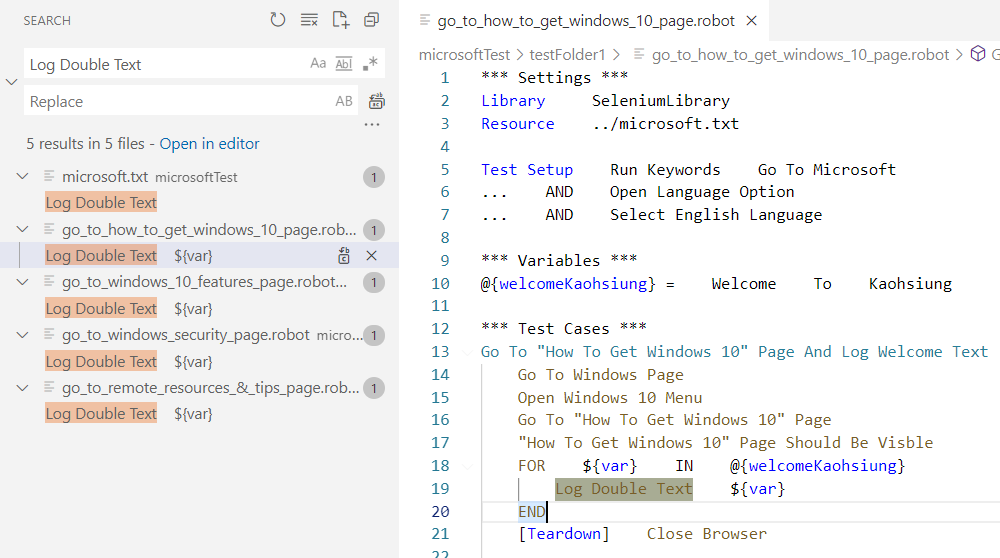
\includegraphics[width=0.9\textwidth]{picture/ch5/vscode_search_in_case1.PNG}
   \caption{重複步驟搜尋結果}
   \label{f5.1}
\end{figure}

%\begin{figure}[H]
%	\centering
%	\begin{minipage}[b]{0.43\textwidth}
%		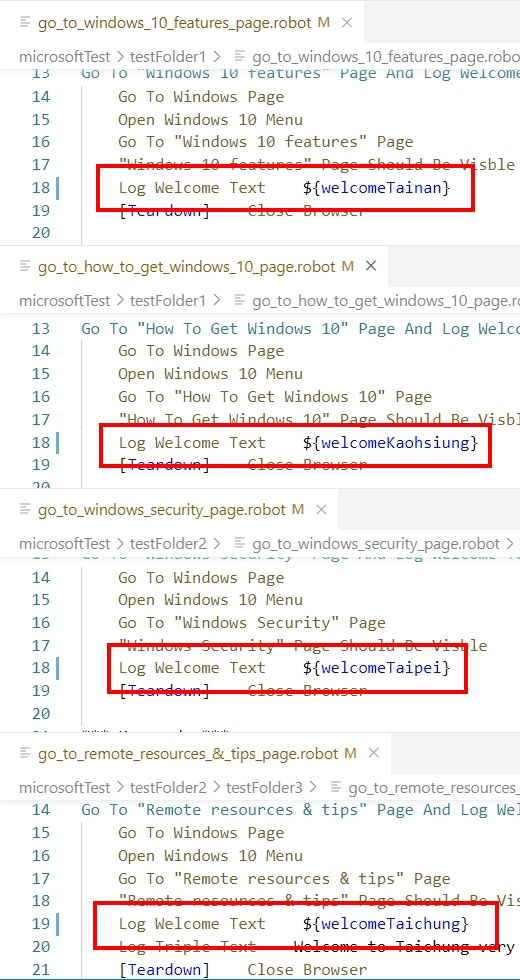
\includegraphics[width=1.05\textwidth]{picture/ch5/After_replace_with_new_keyword_in_case1.png}
%		\caption{關鍵字取代重複步驟後結果}
%		\label{f5.2}
%	\end{minipage}
%	\begin{minipage}[b]{0.53\textwidth}
%		\centering
%		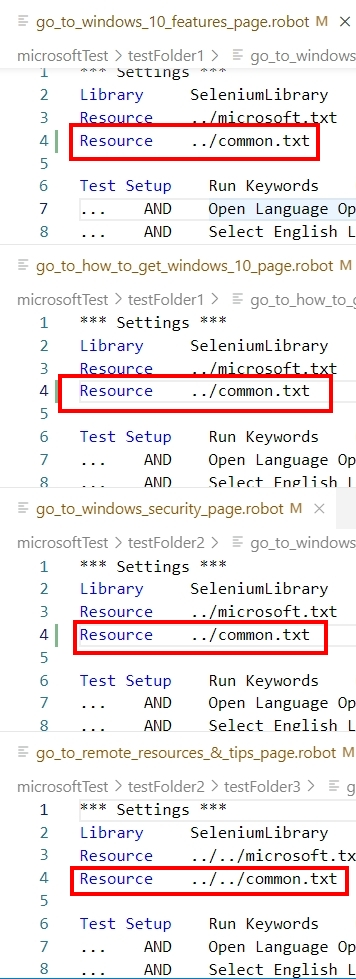
\includegraphics[width=0.85\textwidth]{picture/ch5/Import_resource_in_case1.png}
%		\caption{引入新關鍵字所需之測試資源結果}
%		\label{f5.3}
%	\end{minipage}
%\end{figure}

\subsection{使用擴充後之RF Refactoring}\label{s5.1.2}
\indent
後續使用擴充後之RF Refactoring的Wrap Steps As A New Keyword功能重構\ref{s5.1}節所提及之重複步驟,選取其中一個測試套件中的重複步驟,其將會自動把未宣告於步驟中的變數加入新關鍵字的參數,如圖\ref{f5.4}所示,於此視窗可以同時決定新關鍵字之名稱,並且創立新關鍵字於圖\ref{f5.5}視圖中所選擇之檔案。根據專案下所檢查出含有重複步驟的測試套件,其可在圖\ref{f5.6}之視圖中選擇要以新關鍵字取代之重複步驟,並且為每個要使用的新關鍵字決定其參數實際值,以此完成重複步驟之取代,最後RF Refactoring將自動引入新關鍵字所需之測試資源。

\begin{figure}[H]
    \centering
    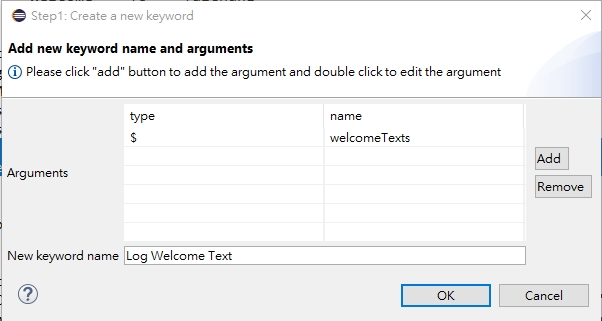
\includegraphics[width=0.7\textwidth]{picture/ch5/Eclipse_create_keyword_in_case1.png}
    \caption{創立新關鍵字視窗結果}
    \label{f5.4}
\end{figure}

\begin{figure}[H]
    \centering
    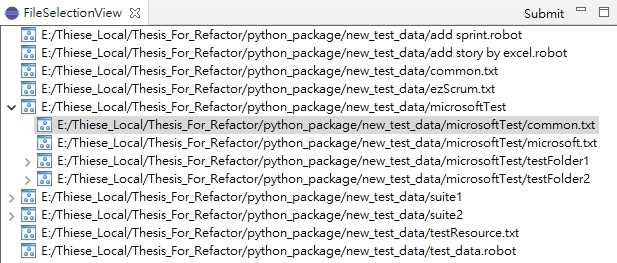
\includegraphics[width=0.7\textwidth]{picture/ch5/Eclipse_choose_file_to_create_keyword_in_case1.png}
    \caption{專案下檔案顯示視圖結果}
    \label{f5.5}
\end{figure}

\begin{figure}[H]
    \centering
    \includegraphics[width=0.7\textwidth]{picture/ch5/Eclipse_choose_duplicate_steps_in_case1.png}
    \caption{搜尋重複步驟結果之視圖}
    \label{f5.6}
\end{figure}

%\begin{figure}[H]
%	\centering
%	\begin{minipage}[b]{0.43\textwidth}
%		\includegraphics[width=1.05\textwidth]{picture/ch5/Eclipse_replace_result_in_case1.png}
%		\caption{關鍵字取代重複步驟後結果}
%		\label{f5.7}
%	\end{minipage}
%	\begin{minipage}[b]{0.53\textwidth}
%		\centering
%		\includegraphics[width=0.85\textwidth]{picture/ch5/Eclipse_Import_resource_result_in_case1.png}
%		\caption{引入新關鍵字所需之測試資源結果}
%		\label{f5.8}
%	\end{minipage}
%\end{figure}

\subsection{重構工具使用之比較}

\begin{table}[H]
    \begin{center}
    \caption{使用兩種工具包裹重複步驟成為新關鍵字並引入所需測試資源之比較}\label{t5.1}
        \begin{tabular}{|c|c|c|}\hline
                             & 使用VSCode重構花費之時間    & 使用擴充後之RF Refactoring重構花費之時間    \\\hline
        測試人員1           & 06m02s          & 03m24s    \\\hline
        測試人員2           & 05m12s          & 04m20s    \\\hline
        測試人員3           & 07m31s          & 04m20s    \\\hline
        測試人員4           & 06m20s          & 04m59s    \\\hline
        測試人員5           & 06m29s          & 06m07s    \\\hline
\textbf{平均時間}           & \textbf{06m18s} & \textbf{04m38s}    \\\hline
        \end{tabular}
    \end{center}
\end{table}
\indent
表\ref{t5.1}為紀錄團隊測試人員使用兩種不同工具進行此重構之比較,從表中可見每一位測試人員根據經驗之不同,使用VSCode進行重構所花費之時間也略微不同,平均大約花費了6分18秒,並且重構過程中,測試人員有三位不小心忽視了新關鍵字所需之測試資源,導致測試失敗;而使用擴充後之RF Refactoring重構時,平均大約花費了4分38秒,並且未有測試資源沒被引入之狀況發生。由此比較可發現,使用擴充後之RF Refactoring進行此重構時,因為不需要手動搜尋重複步驟以及檢查所需之測試資源是否引入,能夠花費較少的時間,其大約減少了26.4\%的時間,並且較不容易發生錯誤。

\section{案例二:移動測試資源中的關鍵字宣告並引入所需測試資源}\label{s5.2}
\indent
程式碼\ref{l5.4}為測試專案的測試套件之一,其中第5行之Go To Microsoft關鍵字於其他測試套件剛好也需要使用,因此必須將其之宣告移動至共用之測試資源,以便其他測試套件使用。在移動到目標測試資源後,必須檢查原先已使用此關鍵字之四個測試套件是否都有引入其所需之測試資源,避免發生未宣告關鍵字之錯誤。

\indent
根據此案例之重構,本論文邀請與\ref{s5.1}節相同之五位測試團隊成員使用下列小節之方式,進行相對應之重構,最後比較其使用差異。

\begin{lstlisting}[caption=前往如何取得Windows10頁面之測試套件, label={l5.4}]
1   *** Settings ***
2   Library     SeleniumLibrary
3   Resource    ../microsoft.txt
4
5   Test Setup    Run Keywords    Go To Microsoft
6   ...    AND    Open Language Option
7   ...    AND    Select English Language

8   *** Variables ***
9   @{welcomeKaohsiung} =    Welcome    To    Kaohsiung
10
11  *** Test Cases ***
12  Go To "How To Get Windows 10" Page And Log Welcome Text
13      Go To Windows Page
14      Open Windows 10 Menu
15      Go To "How To Get Windows 10" Page
16      "How To Get Windows 10" Page Should Be Visible
17      Log Welcome Text    ${welcomeKaohsiung}
18      [Teardown]    Close Browser
\end{lstlisting}

\subsection{使用Visual Studio Code搜尋取代工具}
\indent
首先利用VSCode將需要移動之關鍵字宣告於其所在檔案中移除,並在共用測試資源上完整複製遭移除之關鍵字宣告,後續於搜尋工具之視窗,以被移動之關鍵字名稱進行搜尋,搜尋結果如圖\ref{f5.9}所示,其中一個搜尋結果為關鍵字之宣告的,故不需檢查,其餘結果皆為原先已使用此關鍵字之測試套件。接著於每個測試套件中搜尋是否有引入共用之測試資源,如否則為其引入以避免測試錯誤。

\begin{figure}[H]
    \centering
    \includegraphics[width=0.35\textwidth]{picture/ch5/Search_using_keyword_in_case2.png}
    \caption{搜尋使用被移動關鍵字之測試套件結果}
    \label{f5.9}
\end{figure}

%\begin{figure}[H]
%	\centering
%	\begin{minipage}[b]{0.5\textwidth}
%		\includegraphics[width=0.8\textwidth]{picture/ch5/Import_resource_in_case2.png}
%		\caption{引入關鍵字所需之測試資源結果}
%		\label{f5.10}
%	\end{minipage}
%	\begin{minipage}[b]{0.48\textwidth}
%		\centering
%		\includegraphics[width=1.2\textwidth]{picture/ch5/Move_keyword_result_in_case2.png}
%		\caption{關鍵字宣告移動之結果}
%		\label{f5.11}
%	\end{minipage}
%\end{figure}

\subsection{使用擴充後之RF Refactoring}
\indent
接著使用擴充後之RF Refactoring的Move Keyword Defined To Another File功能重構\ref{s5.2}節所提及的需移動之關鍵字宣告,選取其關鍵字名稱後,即可將關鍵字宣告移動至圖\ref{f5.12}視圖中所選取之目標檔案,後續RF Refactoring將自動為原先已使用此關鍵字之測試套件引入所需測試資源。

\begin{figure}[H]
    \centering
    \includegraphics[width=0.7\textwidth]{picture/ch5/Eclipse_choose_file_in_case2.png}
    \caption{專案下全部測試檔案之視圖}
    \label{f5.12}
\end{figure}

%\begin{figure}[H]
%	\centering
%	\begin{minipage}[b]{0.48\textwidth}
%		\centering
%		\includegraphics[width=0.9\textwidth]{picture/ch5/Eclipse_import_resource_in_case2.png}
%		\caption{引入關鍵字所需測試資源之結果}
%		\label{f5.13}
%	\end{minipage}
%	\begin{minipage}[b]{0.5\textwidth}
%		\includegraphics[width=1.2\textwidth]{picture/ch5/Eclipse_move_keyword_result_in_case2.png}
%		\caption{關鍵字宣告移動之結果}
%		\label{f5.14}
%	\end{minipage}
%\end{figure}

\subsection{重構工具使用之比較}

\begin{table}[H]
    \begin{center}
    \caption{使用兩種工具移動關鍵字宣告並引入所需測試資源之比較}\label{t5.2}
        \begin{tabular}{|c|c|c|}\hline
                & 使用VSCode重構花費之時間 & 使用擴充後之RF Refactoring重構花費之時間    \\\hline
        測試人員1      & 01m14s             & 00m26s    \\\hline
        測試人員2      & 01m35s             & 00m18s    \\\hline
        測試人員3      & 01m17s             & 00m22s    \\\hline
        測試人員4      & 01m00s             & 00m26s    \\\hline
        測試人員5      & 02m02s             & 00m41s    \\\hline
\textbf{平均時間}      & \textbf{01m25s}    & \textbf{00m26s}    \\\hline
        \end{tabular}
    \end{center}
\end{table}
\indent
表\ref{t5.2}為紀錄團隊測試人員使用兩種不同工具進行此重構之比較,從表中可發現,使用VSCode進行重構時,平均花費了1分25秒,且有兩位測試人員對於部分測試套件有錯誤引入關鍵字所需測試資源之相對路徑,導致測試錯誤;而使用擴充後之RF Refactoring重構時,平均花費了26秒,且引入所需測試資源之路徑皆為正確。從此比較可發現,使用擴充後之RF Refactoring進行此重構時,因為不需要自我檢查測試套件是否都有引入所需之測試資源,能夠花費較少的時間,其大約減少了69.4\%的時間,並且較不容易因人為檢查缺漏而發生錯誤。
% \chapter{結論與未來展望}
\section{結論}
\indent
本論文擴充了劉冠志論文\cite{LIU-Thesis}於Eclipse實作之外掛程式RF Refactoring,增加了兩種重構方法,不只讓團隊於選擇重構方法時能夠更加多元,且能夠減少搜尋的缺漏及取代的錯誤。根據第三章RF Refactoring延伸功能之設計,使擴充後的RF Refactoring在搜尋重複步驟時,能夠確實地得到需要進行新關鍵字取代之重複步驟,而不是得到與團隊需求不同之步驟;此外移動關鍵字宣告後,其搜尋原先使用關鍵字之測試腳本時,也能夠確實地得到真正有使用被移動之關鍵字的測試腳本,而不是得到使用類似名稱之關鍵字的測試腳本等等。

\indent
第四章中將擴充之重構功能結合至原先已存在之外掛程式RF Refactoring後,使用者不必進行搜尋,即可得知其需要被取代的重複步驟,並且可以依照需求進行選擇,而移動關鍵字宣告後,也不需要自行引入測試腳本所需之測試資源,即可完成重構。由第五章中可得知,當團隊遇到實際案例時的重構過程,並且使用擴充後之RF Refactoring,確實可以減少重構之時間,因而提升整體重構效率,此外,案例中的測試專案規模較小,能夠減少重構的時間也相對較少,如果將擴充後之RF Refactoring應用於規模更加龐大的測試專案,其能夠減少的重構時間也能夠相對上升。
\newpage

\section{未來方向}
\indent
本論文擴充之測試腳本重構工具仍有待改善之處,以下將分為三點說明:

\begin{itemize}

\item\textbf{執行重構之效能:}
本論文擴充之測試腳本重構工具在執行任一重構方法前,都必須先行解析測試專案下的所有測試資料,而使用者通常必須花費較長時間等待其解析完成,並且專案中的資料越多時,則等待時間也會相對增加。若能在啟動重構工具時,利用其他執行緒事先於背景解析專案下之測試資料,且資料有任何新增、修改、刪除等操作時,則再次重新解析相對應資料,確保檔案內容之正確,即可消除執行重構方法時的等待時間,使重構效率更加提升。

\item\textbf{重構方法之新增:}
測試腳本重構工具經本論文擴充後,其重構方法目前有五個,重新命名關鍵字、重新命名變數、修改關鍵字介面、包裹重複步驟成為新關鍵字及移動關鍵宣告,重構方法擁有十分多種,而測試人員於開發時,也會有遭遇其他重構需求的時候,因此如果能夠增加更多種類之重構方法,其能減少測試人員於手動重構時錯誤及缺漏的產生,表\ref{t6.1}為未來可擴充之重構方法。

\item\textbf{其他功能:}
本論文所擴充之測試腳本重構工具是參考其他IDE重構功能所開發,因此於重構完成後必須手動執行被重構之測試腳本,才可知道其是否測試功能與未重構前相同,若能與其他測試腳本變更偵測工具結合,例如:邱文煜論文\cite{CHIU-Thesis}所提供之測試選擇工具,於重構完成後,即可執行有所變更之測試腳本,能夠更快地知道重構後之結果是否如測試人員所需,縮短測試人員於重構後之確認時間。

\end{itemize}

\begin{table}[H]
    \begin{center}
    \caption{未來可擴充之重構方法}\label{t6.1}
        \begin{tabular}{|c|l|}\hline
        可擴充之重構方法           & \multicolumn{1}{c|}{重構方法之描述}    \\\hline
        抽取變數                 & 搜尋出多個重複數值並建立新變數進行取代。    \\\hline
        移動變數                 & 移動變數宣告至其他測試資源中,並確保引入所需測試資源。    \\\hline
        內聯化(Inline)關鍵字      & 刪除關鍵字宣告並將使用其的參考以關鍵字的實作取代。    \\\hline
        內聯化(Inline)變數        & 刪除變數宣告並將使用其的參考以變數的實作取代。    \\\hline
        重新命名測試檔案           & 重新命名測試檔案,且確保原先引入此檔案之資訊正確。    \\\hline
        \end{tabular}
    \end{center}
\end{table} 
\vfill
\newpage
\addcontentsline{toc}{chapter}{參考文獻}

\bibliographystyle{unsrt}
\bibliography{reference}

\end{document}